\documentclass[twocolumn]{scrartcl}

%%%%%%%%%%%%%%%%%%%%%%%%%%%%%%%%%%%%%%%
%% Makros & anderer Low-Level bastel %%
%%%%%%%%%%%%%%%%%%%%%%%%%%%%%%%%%%%%%%%
\makeatletter
%% Makros für Titel, Autor und Datum 
%% Dank diesem Makro stehen Titel, Autor und Datum überall im Dokument zur verfügung
%% Date hat zudem den Default-Wert \today
\def\@Title{}
\def\@Author{}
\def\@Date{\today}
\newcommand{\Title}{\@Title}
\newcommand{\Author}{\@Author}
\newcommand{\Date}{\@Date}
\AtBeginDocument{%
  \let\@Title\@title
  \let\@Author\@author
  \let\@Date\@date
}

%% Makros für den Arraystretch (bei uns meist in Tabellen genutzt, welche Formeln enthalten)
% Default Value
\def\@ArrayStretchDefault{1} % Entspricht der Voreinstellung von Latex

% Setzt einen neuen Wert für den arraystretch
\newcommand{\setArrayStretch}[1]{\renewcommand{\arraystretch}{#1}}

% Setzt den arraystretch zurück auf den default wert
\newcommand{\resetArrayStretch}{\renewcommand{\arraystretch}{\@ArrayStretchDefault}}

% Makro zum setzten des Default arraystretch. Kann nur in der Präambel verwendet werden.
\newcommand{\setDefaultArrayStretch}[1]{%
	\AtBeginDocument{%
		\def\@ArrayStretchDefault{#1}
		\renewcommand{\arraystretch}{#1}
	}
}
\makeatother


%%%%%%%%%%%%%%%%%%%%%%%
%% Wichtige Packages %%
%%%%%%%%%%%%%%%%%%%%%%%
\usepackage[utf8]{inputenc} % UTF-8 unterstützung
\usepackage[english, ngerman]{babel} % Silbentrennung
\usepackage[automark]{scrpage2} % Header und Footer
\usepackage{tabularx}

% Für Abbildungen mit mehreren kleinen Bilder
% Doku: http://www.ctan.org/tex-archive/macros/latex/contrib/caption/
\usepackage{caption}
\usepackage{subcaption}

\ifx \GUARDhsrColors \undefined
\def\GUARDhsrColors{}

\usepackage[table]{xcolor}

\definecolor{HSRWhite}{cmyk}{0,0,0,0}

\definecolor{HSRBlue}{cmyk}{1,0.4,0,0.2}
\definecolor{HSRBlue80}{cmyk}{0.8,0.32,0,0.16}
\definecolor{HSRBlue60}{cmyk}{0.6,0.24,0,0.12}
\definecolor{HSRBlue40}{cmyk}{0.4,0.16,0,0.08}
\definecolor{HSRBlue20}{cmyk}{0.2,0.08,0,0.04}

\definecolor{HSRLightGray}{cmyk}{0,0,0,0.30}
\definecolor{HSRLightGray80}{cmyk}{0,0,0,0.24}
\definecolor{HSRLightGray60}{cmyk}{0,0,0,0.18}
\definecolor{HSRLightGray40}{cmyk}{0,0,0,0.12}
\definecolor{HSRLightGray20}{cmyk}{0,0,0,0.06}

\definecolor{HSRSchwarz}{cmyk}{0,0,0,1}
\definecolor{HSRSchwarz80}{cmyk}{0,0,0,0.8}
\definecolor{HSRSchwarz60}{cmyk}{0,0,0,0.6}
\definecolor{HSRSchwarz40}{cmyk}{0,0,0,0.4}
\definecolor{HSRSchwarz20}{cmyk}{0,0,0,0.2}

\definecolor{HSRHematite}{cmyk}{0.6,1,0.4,0.2}
\definecolor{HSRHematite80}{cmyk}{0.48,0.80,0.32,0.16}
\definecolor{HSRHematite60}{cmyk}{0.36,0.60,0.24,0.12}
\definecolor{HSRHematite40}{cmyk}{0.24,0.40,0.16,0.08}
\definecolor{HSRHematite20}{cmyk}{0.12,0.20,0.08,0.04}

\definecolor{HSRLakeGreen}{cmyk}{0.70,0.30,0.45,0.05}
\definecolor{HSRLakeGreen80}{cmyk}{0.56,0.24,0.36,0.03}
\definecolor{HSRLakeGreen60}{cmyk}{0.42,0.18,0.27,0.02}
\definecolor{HSRLakeGreen40}{cmyk}{0.28,0.06,0.13,0.06}
\definecolor{HSRLakeGreen20}{cmyk}{0.14,0.06,0.09,0.01}

\definecolor{HSRReed}{cmyk}{0.10,0.25,0.45,0.60}
\definecolor{HSRReed80}{cmyk}{0.08,0.20,0.36,0.48}
\definecolor{HSRReed60}{cmyk}{0.06,0.15,0.27,0.36}
\definecolor{HSRReed40}{cmyk}{0.04,0.10,0.18,0.24}
\definecolor{HSRReed20}{cmyk}{0.02,0.05,0.09,0.12}

\definecolor{HSRPetrol}{cmyk}{1,0.18,0,0.45}
\definecolor{HSRPetrol80}{cmyk}{0.64,0.08,0.12,0.32}
\definecolor{HSRPetrol60}{cmyk}{0.48,0.06,0.09,0.24}
\definecolor{HSRPetrol40}{cmyk}{0.32,0.04,0.06,0.16}
\definecolor{HSRPetrol20}{cmyk}{0.16,0.02,0.03,0.08}

\definecolor{HSRBasswood}{cmyk}{0.25,0.05,0.70,0.15}
\definecolor{HSRBasswood80}{cmyk}{0.20,0.04,0.56,0.12}
\definecolor{HSRBasswood60}{cmyk}{0.15,0.03,0.42,0.09}
\definecolor{HSRBasswood40}{cmyk}{0.10,0.02,0.28,0.06}
\definecolor{HSRBasswood20}{cmyk}{0.05,0.01,0.14,0.03}


\fi
\ifx\GUARDmathe\undefined
\def\GUARDmathe{}

\usepackage{amssymb}
% Das mathtools package ist eine Erweiterung zum amsmath package.
% Das amsmath package wird dabei automatisch geladen
\usepackage{mathtools}


% Package mit vielen weiteren Mathe Symbolen
% http://www.ctan.org/tex-archive/fonts/mathabx
\usepackage{mathabx}

% This package defines commands to access bold math symbols. The basic command
% is \bm which may be used to make the math expression in its argument be typeset
% using bold fonts.
\usepackage{bm}

\fi
\ifx\GUARDenumitem\undefined
\def\GUARDenumitem{}

\usepackage{enumitem}

\fi

% Seitenränder für Formelsammlungen
\usepackage[left=0.5cm,right=0.5cm,top=0.5cm,bottom=0.5cm,includeheadfoot]{geometry}

\usepackage{multirow} % Create tabular cells spanning multiple rows
\usepackage{multicol} % In­ter­mix sin­gle and mul­ti­ple columns
\usepackage{rotating} % Rotation tools, including rotated fullpage floats


%%%%%%%%%%%%%%%%%%%%%%%%%%%%%%%%%%%
%% Layout der Kopf und Fusszeile %%
%%%%%%%%%%%%%%%%%%%%%%%%%%%%%%%%%%%
\deftripstyle{zusammenfassung}[0pt][0.5pt]
	{\Title}	% Kopfzeile innen
	{\headmark}	% Kopfzeile mitte
	{\pagemark}	% Kopfzeile aussen
	{\Author}	% Fusszeile innen
	{
\includegraphics[width=1.6cm]{./header/lizenzen/cc-by-nc-sa/small.png}}			% Fusszeile mitte
	{\Date}	% Fusszeile aussen
\pagestyle{zusammenfassung}



% Makros für Verweise auf ein Buch oder Skript
\newcommand{\buch}[1]{\texorpdfstring{$_{\textcolor{HSRLakeGreen}{\mbox{\small{#1}}}}$}{}}
\newcommand{\buchSeite}[1]{\texorpdfstring{\ensuremath{_{\textcolor{red}{\mbox{\small{ S#1}}}}}}{}}
\newcommand{\skript}[1]{\texorpdfstring{$_{\textcolor{HSRReed}{\mbox{\small{#1}}}}$}{}}
\newcommand{\formelbuch}[1]{$_{\textcolor{red}{\mbox{\small{S#1}}}}$}

% Zeilenhöhe Tabellen:
\newcommand{\arraystretchOriginal}{1.5}
\renewcommand{\arraystretch}{\arraystretchOriginal}

\setlength{\parindent}{0pt}
\ifx\GUARDhyperref\undefined
\def\GUARDhyperref{}

\ifx \GUARDhsrColors \undefined
\def\GUARDhsrColors{}

\usepackage[table]{xcolor}

\definecolor{HSRWhite}{cmyk}{0,0,0,0}

\definecolor{HSRBlue}{cmyk}{1,0.4,0,0.2}
\definecolor{HSRBlue80}{cmyk}{0.8,0.32,0,0.16}
\definecolor{HSRBlue60}{cmyk}{0.6,0.24,0,0.12}
\definecolor{HSRBlue40}{cmyk}{0.4,0.16,0,0.08}
\definecolor{HSRBlue20}{cmyk}{0.2,0.08,0,0.04}

\definecolor{HSRLightGray}{cmyk}{0,0,0,0.30}
\definecolor{HSRLightGray80}{cmyk}{0,0,0,0.24}
\definecolor{HSRLightGray60}{cmyk}{0,0,0,0.18}
\definecolor{HSRLightGray40}{cmyk}{0,0,0,0.12}
\definecolor{HSRLightGray20}{cmyk}{0,0,0,0.06}

\definecolor{HSRSchwarz}{cmyk}{0,0,0,1}
\definecolor{HSRSchwarz80}{cmyk}{0,0,0,0.8}
\definecolor{HSRSchwarz60}{cmyk}{0,0,0,0.6}
\definecolor{HSRSchwarz40}{cmyk}{0,0,0,0.4}
\definecolor{HSRSchwarz20}{cmyk}{0,0,0,0.2}

\definecolor{HSRHematite}{cmyk}{0.6,1,0.4,0.2}
\definecolor{HSRHematite80}{cmyk}{0.48,0.80,0.32,0.16}
\definecolor{HSRHematite60}{cmyk}{0.36,0.60,0.24,0.12}
\definecolor{HSRHematite40}{cmyk}{0.24,0.40,0.16,0.08}
\definecolor{HSRHematite20}{cmyk}{0.12,0.20,0.08,0.04}

\definecolor{HSRLakeGreen}{cmyk}{0.70,0.30,0.45,0.05}
\definecolor{HSRLakeGreen80}{cmyk}{0.56,0.24,0.36,0.03}
\definecolor{HSRLakeGreen60}{cmyk}{0.42,0.18,0.27,0.02}
\definecolor{HSRLakeGreen40}{cmyk}{0.28,0.06,0.13,0.06}
\definecolor{HSRLakeGreen20}{cmyk}{0.14,0.06,0.09,0.01}

\definecolor{HSRReed}{cmyk}{0.10,0.25,0.45,0.60}
\definecolor{HSRReed80}{cmyk}{0.08,0.20,0.36,0.48}
\definecolor{HSRReed60}{cmyk}{0.06,0.15,0.27,0.36}
\definecolor{HSRReed40}{cmyk}{0.04,0.10,0.18,0.24}
\definecolor{HSRReed20}{cmyk}{0.02,0.05,0.09,0.12}

\definecolor{HSRPetrol}{cmyk}{1,0.18,0,0.45}
\definecolor{HSRPetrol80}{cmyk}{0.64,0.08,0.12,0.32}
\definecolor{HSRPetrol60}{cmyk}{0.48,0.06,0.09,0.24}
\definecolor{HSRPetrol40}{cmyk}{0.32,0.04,0.06,0.16}
\definecolor{HSRPetrol20}{cmyk}{0.16,0.02,0.03,0.08}

\definecolor{HSRBasswood}{cmyk}{0.25,0.05,0.70,0.15}
\definecolor{HSRBasswood80}{cmyk}{0.20,0.04,0.56,0.12}
\definecolor{HSRBasswood60}{cmyk}{0.15,0.03,0.42,0.09}
\definecolor{HSRBasswood40}{cmyk}{0.10,0.02,0.28,0.06}
\definecolor{HSRBasswood20}{cmyk}{0.05,0.01,0.14,0.03}


\fi

\usepackage[plainpages=false,pdfpagelabels]{hyperref}
\hypersetup{
  pdfstartview={FitH}, % fits the width of the page to the window
  pdfauthor={\Author},
  pdfcreator={\Author},
  pdfproducer={\Author},
  pdftitle={\Title},
  colorlinks=true,
  linkcolor=HSRBlue,
  citecolor=HSRReed,
  filecolor=HSRLake,
  urlcolor=HSRHematite
}

\fi


\title{MatAuf}
\author{H. Badertscher, M. Ehrler, L. Leuenberger}

\renewcommand{\arraystretch}{1.2}

\let\olditemize\itemize
\renewcommand{\itemize}{\olditemize\setlength{\itemsep}{0pt}}

% Everything compact as posssible
\setitemize{noitemsep,topsep=0pt,parsep=0pt,partopsep=0pt}
\usepackage[compact]{titlesec}
\titlespacing{\section}{0pt}{0.5ex}{0ex}
\titlespacing{\subsection}{0pt}{0.5ex}{0ex}
\titlespacing{\subsubsection}{0pt}{0.5ex}{0ex}
\setlength{\parskip}{0cm}
\setlength{\parindent}{0em}
\setlength{\intextsep}{0ex}
\setlength{\itemsep}{0ex}
\setlength{\dbltextfloatsep}{0ex}
\setlength{\textfloatsep}{0ex}
\setlength{\dblfloatsep}{0ex}
\setlength{\multicolsep}{0ex}
\linespread{0.9}
\setlist[enumerate]{itemsep=0mm}

% Chemistry formulas
\usepackage{chemfig}

% Four pages on one
%\usepackage{pgfpages}
%\pgfpagesuselayout{4 on 1}[a4paper]

\begin{document}

\section{Aufbau der Stoffe}

\subsection{Bindungsarten}
\begin{itemize}
	\item Kovalente Bindung (Atombindung)
		\begin{itemize}
			\item 2 nichtmetallische Atome
			\item Moleküle
		\end{itemize}
	\item Ionenbindung
		\begin{itemize}
			\item Elektrostatische Anziehung zwischen pos. (Kation) und neg. (Anion) geladenem Ion
			\item Ionengitter (Salze)
		\end{itemize}
	\item Metallbindung
		\begin{itemize}
			\item Elektrostatische Anzehung zwischen met. Kation und delokalisiertem Elektron
			\item Kationengitter (Metalle und Legierungen)
		\end{itemize}
\end{itemize}

\subsection{Stoffklassen}
\begin{itemize}
	\item Flüchtige Stoffe (molekulare Stoffe und Edelgase)
	\begin{itemize}
	    \item \textbf{Eigenschaften:} tiefe Schmelz- und Siedetemperatur, nicht leitend, weich
	    \item \textbf{Aufbau:} Molekül (abgeschlossener Atomverband aus Nichtmetallatomen), Edelgase kommen atomar vor
	    \item \textbf{Bindungsart:} Atombindung, gemeinsames Elektronenpaar zw. neutralen Nichtmetallatomen
	    \item \textbf{Beispiel:} $CO_2$, $I_2$, $CH_3CH_2OH$
	\end{itemize}
	\item Salzartige Stoffe
	\begin{itemize}
	    \item \textbf{Eigenschaften:} hohe Schmelz- und Siedetemperatur, im flüssigen oder gelösten Zustand leitend, als Feststoff hart und spröde
	    \item \textbf{Aufbau:} bestehen aus Ionen, die ein unendlich grosses 3-dimensionales Gitter bilden
	    \item \textbf{Bindungsart:} Ionenbindung, elektrostatische Anziehung (Coulomb-Kraft) zwischen Kationen und Anionen
	    \item \textbf{Beispiel:} $CaCO_3$, $CaSO_4$, $Na_2CO_3$
	\end{itemize}
	\item Metallische Stoffe
	\begin{itemize}
	    \item \textbf{Eigenschaften:} elektrisch leitend, metallischer Glanz, häufig hohe Schmelz- und Siedetemperaturen, verformbar, gute Wärmeleiter
	    \item \textbf{Aufbau:} Metallkationen, die ein unendlich grosses 3-dimensionales Gitter bilden, sind von Elektronengas umgeben
	    \item \textbf{Bindungsart:} Metallbindung, elektrostatische Anziehung (Coulomb-Kraft) zwischen Kationen und Elektronengas
	    \item \textbf{Beispiel:} Metalle und Legierungen (Messing, Stahl, Amalgam)
	\end{itemize}
	\item Hochmolekulare Stoffe (Polymere)
	\begin{itemize}
	    \item \textbf{Eigenschaften:} sehr hart, sehr hohe Schmelz- und Siedetemperatur, nicht leitend
	    \item \textbf{Aufbau:} Atomgitter, die sowohl Nichtmetall- als auch Metallatome enthalten können
	    \item \textbf{Bindungsart:} Atombindung, Ionenbindung
	    \item \textbf{Beispiel:} $C$, $SiO_2$, $Al_2O_3$
	\end{itemize}
	\item Diamantartige Stoffe
	\begin{itemize}
	    \item \textbf{Eigenschaften:} keine definierte Schmelztemperatur sondern allmähliches Erweichen, kein Verdampfen sondern Zersetzung
	    \item \textbf{Aufbau:} sehr lange Moleküle, die aus Atomgruppen (Monomeren) bestehen
	    \item \textbf{Bindungsart:} Atombindung
	    \item \textbf{Beispiel:} Kunstoffe (Nylon, PVC, PET, Silikon), natürliche Polymere (Eiweiss, Stärke, DNA)
	\end{itemize}
\end{itemize}

\subsection{Stoffmengen und Stoffmassen}
$1$ $mol$ entsprechen $6.02 \cdot 10^{23}$ Stoffteilchen. Die Zahl $6.02 \cdot 10^{23}$ wird als Avogadro-Zahl $N_A$ bezeichnet.

\subsubsection{Molare Masse}
Die molare Masse $M$ ist die Masse von $1$ $mol$ eines Stoffes. \\
$M=\frac{m}{n}$ \ \ $[M]=\frac{g}{mol}$

\subsection{Kristallstrukturen}
\begin{itemize}
	\item Kristalline Feststoffe (regelmässige Anordnung = Fernordnung), z.B. Metalle, Salze, diamantartige
	\item Amorphe Feststoffe (unregelmässige Anordnung = Nahordnung), z.B. Kunststoffe, Glas
\end{itemize}

\subsubsection{Das Harte-Kugeln-Modell}
\begin{figure}[htbp]
	\begin{subfigure}{0.49\linewidth}
		\centering
		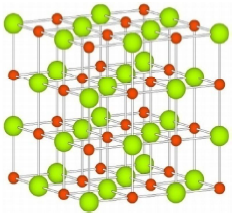
\includegraphics[width=0.49\linewidth]{images/1_Raumgittermodell.png}
		\caption{Raumgittermodell}
	\end{subfigure}
	\begin{subfigure}{0.49\linewidth}
		\centering
		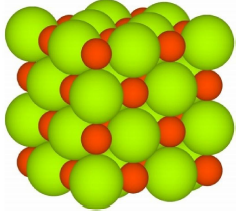
\includegraphics[width=0.49\linewidth]{images/1_Kugelpackungsmodell.png}
		\caption{Kugelpackungsmodell}
	\end{subfigure}
\end{figure}

\subsection{Dichteste Kugelpackungen}
\begin{figure}[htbp]
	\begin{subfigure}{0.49\linewidth}
		\centering
		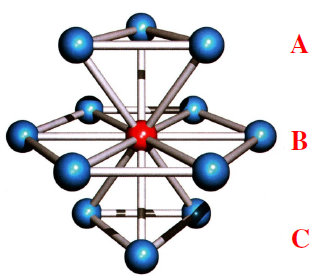
\includegraphics[width=0.49\linewidth]{images/1_kubisch_dichteste_KuPa.png}
		\caption{Kubisch dichteste Kugelpackung}
	\end{subfigure}
	\begin{subfigure}{0.49\linewidth}
		\centering
		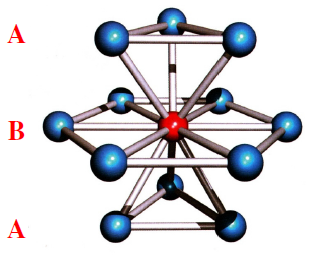
\includegraphics[width=0.49\linewidth]{images/1_hexagonal_dichteste_KuPa.png}
		\caption{Hexagonal dichteste Kugelpackung}
	\end{subfigure}
\end{figure}

\subsubsection{Lücken}
\begin{itemize}
	\item Oktaederlücken: oktaedrisch von 6 Atomen umgeben
	\item Tetraederlücken: tetraedrisch von 4 Atomen umgeben
	\item Koordinationszahl (KZ): Zahl der nächsten Nachbarteilchen (12 bei  dichtester Kugelpackung)
\end{itemize}

\subsection{Elementarzelle}
Kleinste Einheit einer Kristallstruktur. Erlaubt eindeutige Beschreibung des atomaren Aufbaus. 

\begin{multicols}{2}
    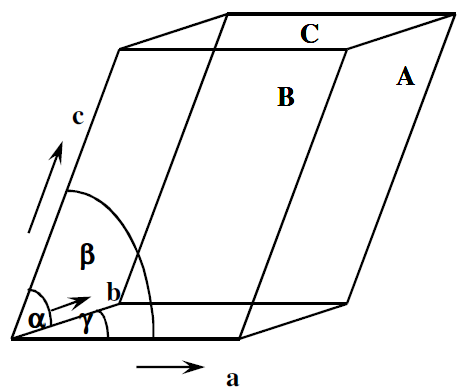
\includegraphics[width=2.5cm]{images/1_Elementarzelle.png}
    
\columnbreak

    Durch 6 Gitterparameter $a$, $b$, $c$, $\alpha$, $\beta$, $\gamma$ eindeutig bestimmt. Es existieren 14 Arten von Elementarzellen. Die drei häufigsten sind: \\
\end{multicols}

\begin{figure}[htbp]
	\begin{subfigure}{0.32\linewidth}
		\centering
		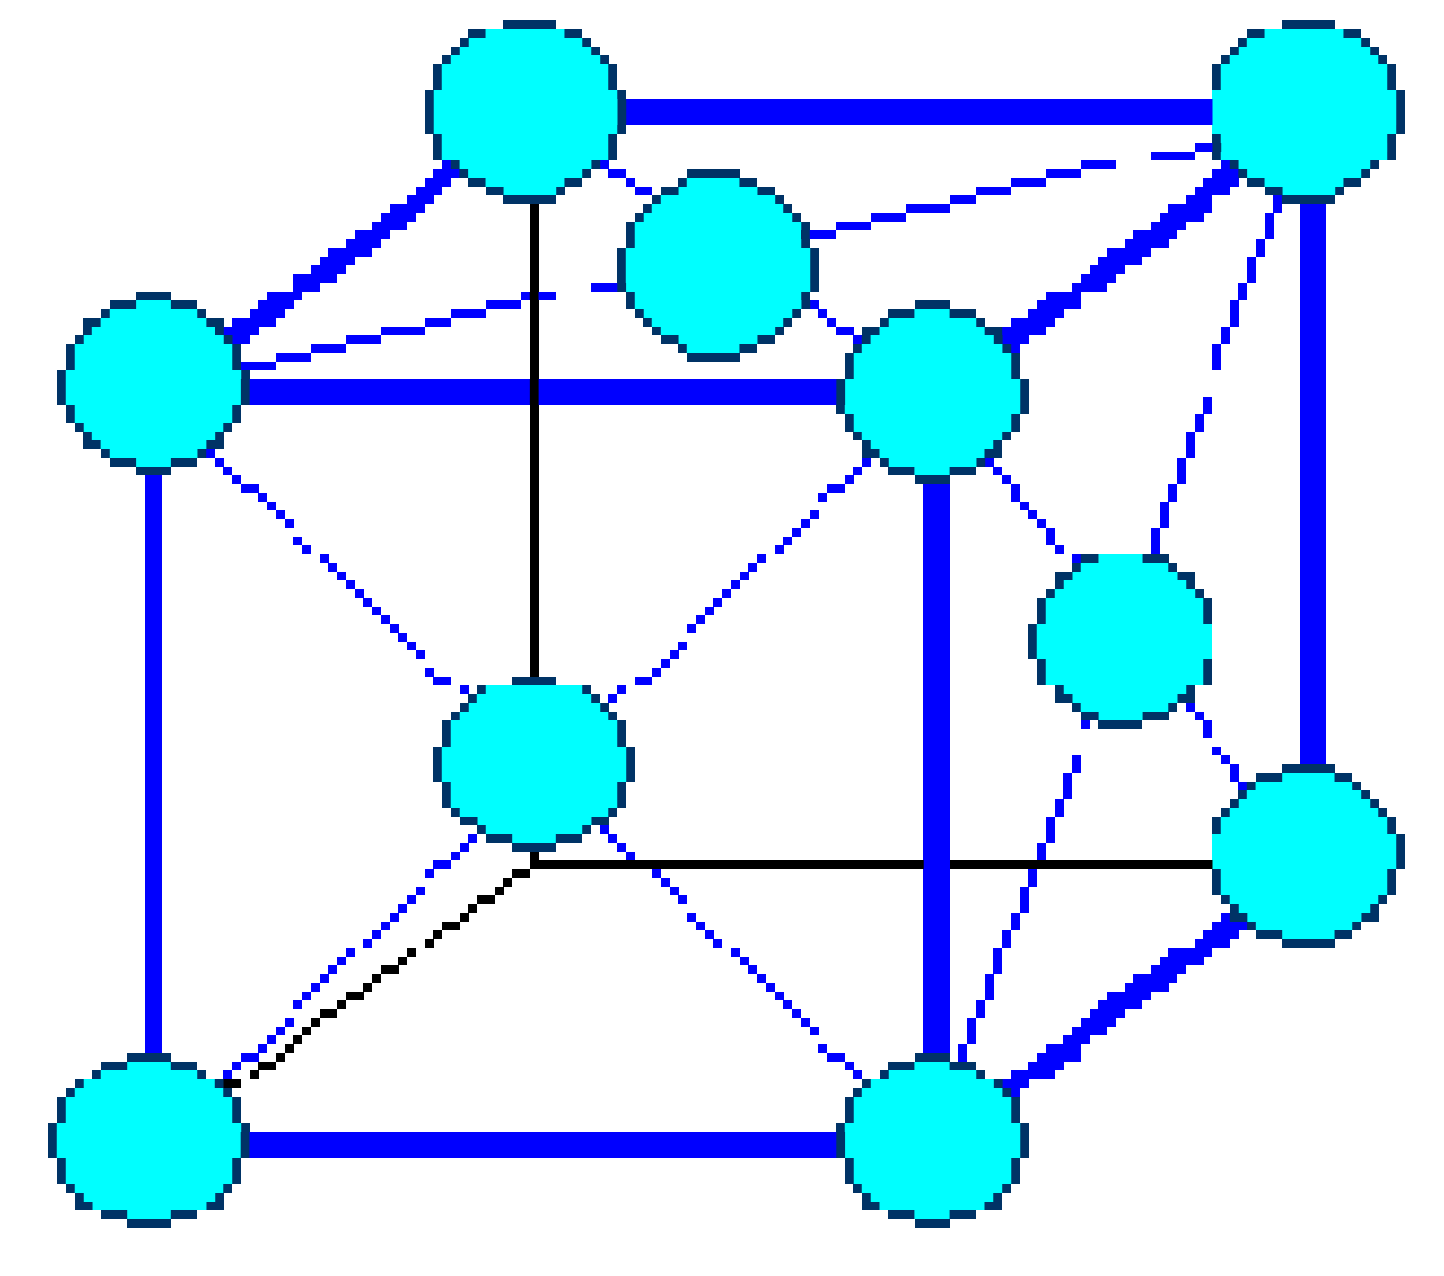
\includegraphics[width=0.5\linewidth]{images/1_kfz.png}
		\caption{kubisch flächenzentriert}
	\end{subfigure}
	\begin{subfigure}{0.32\linewidth}
		\centering
		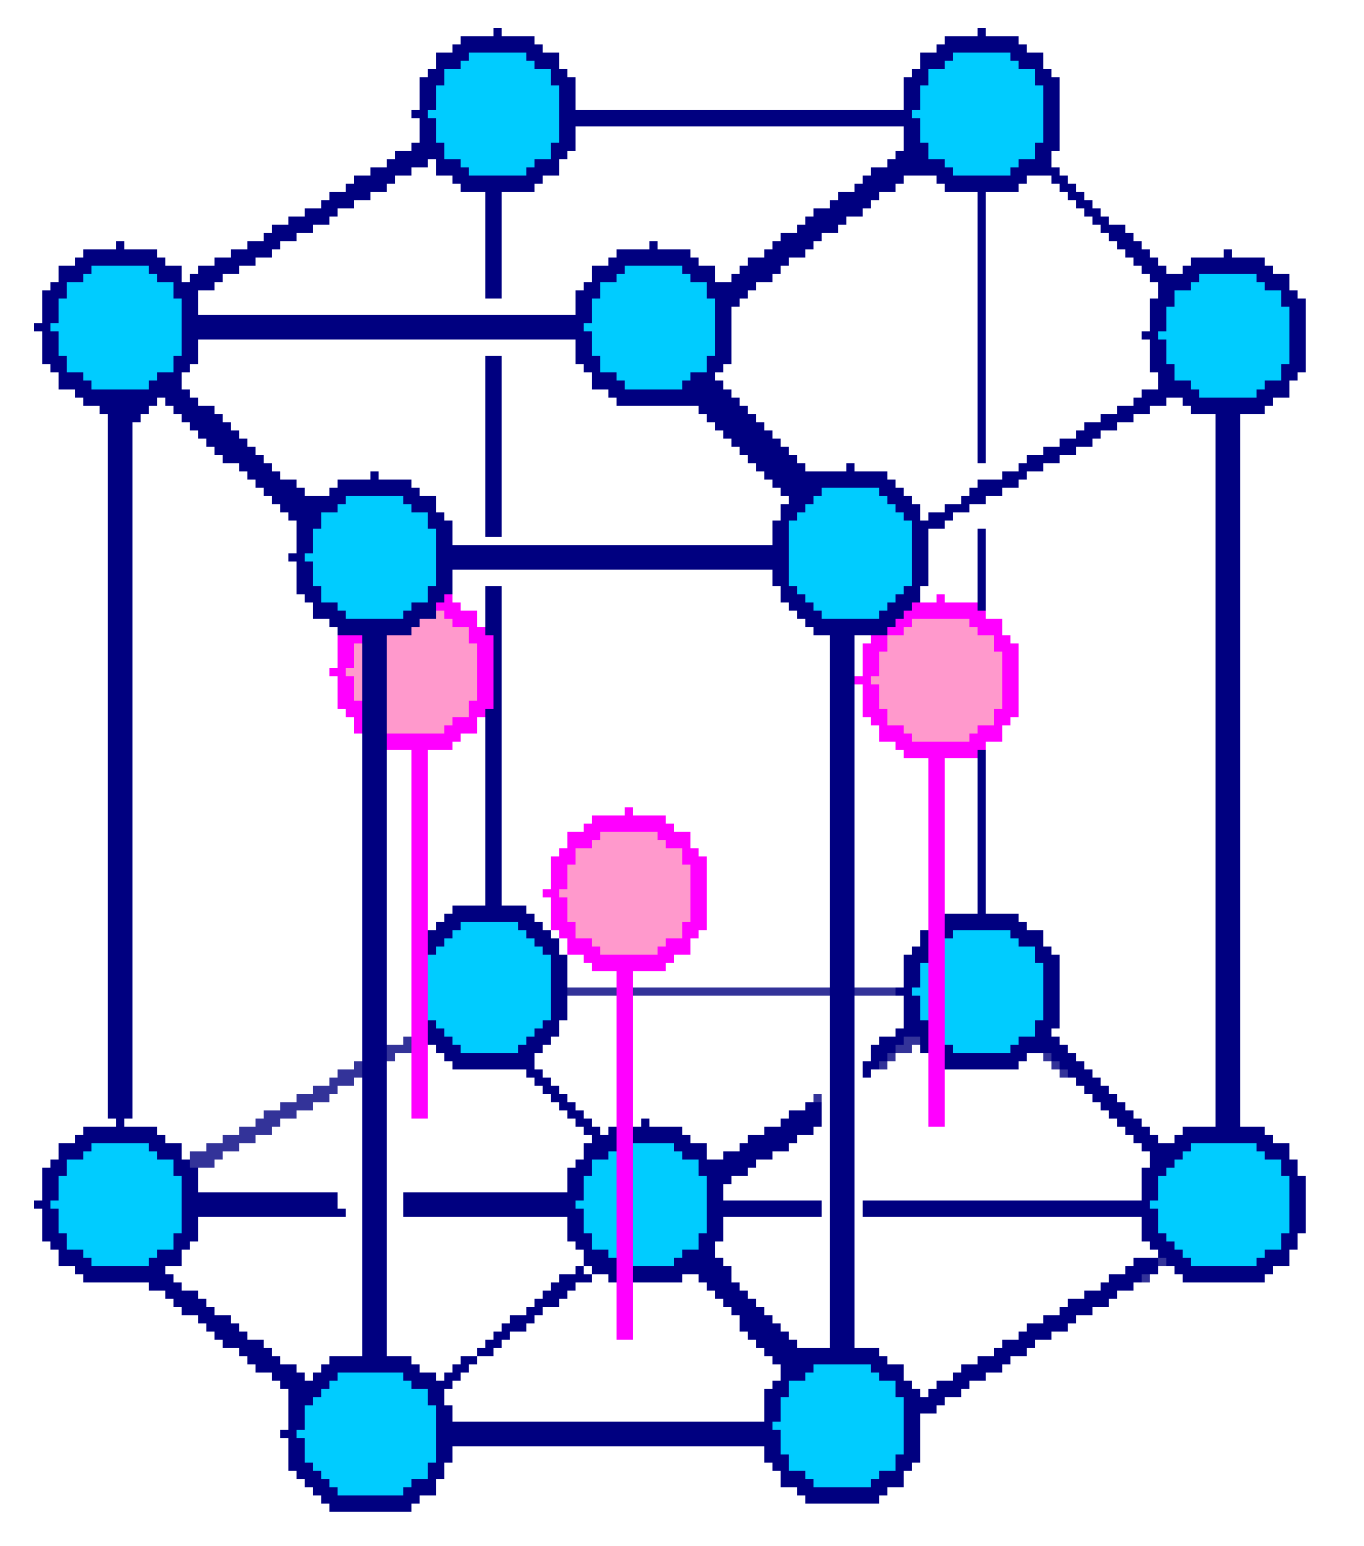
\includegraphics[width=0.5\linewidth]{images/1_hcp.png}
		\caption{hexagonal dichtest gepackt}
	\end{subfigure}
	\begin{subfigure}{0.32\linewidth}
		\centering
		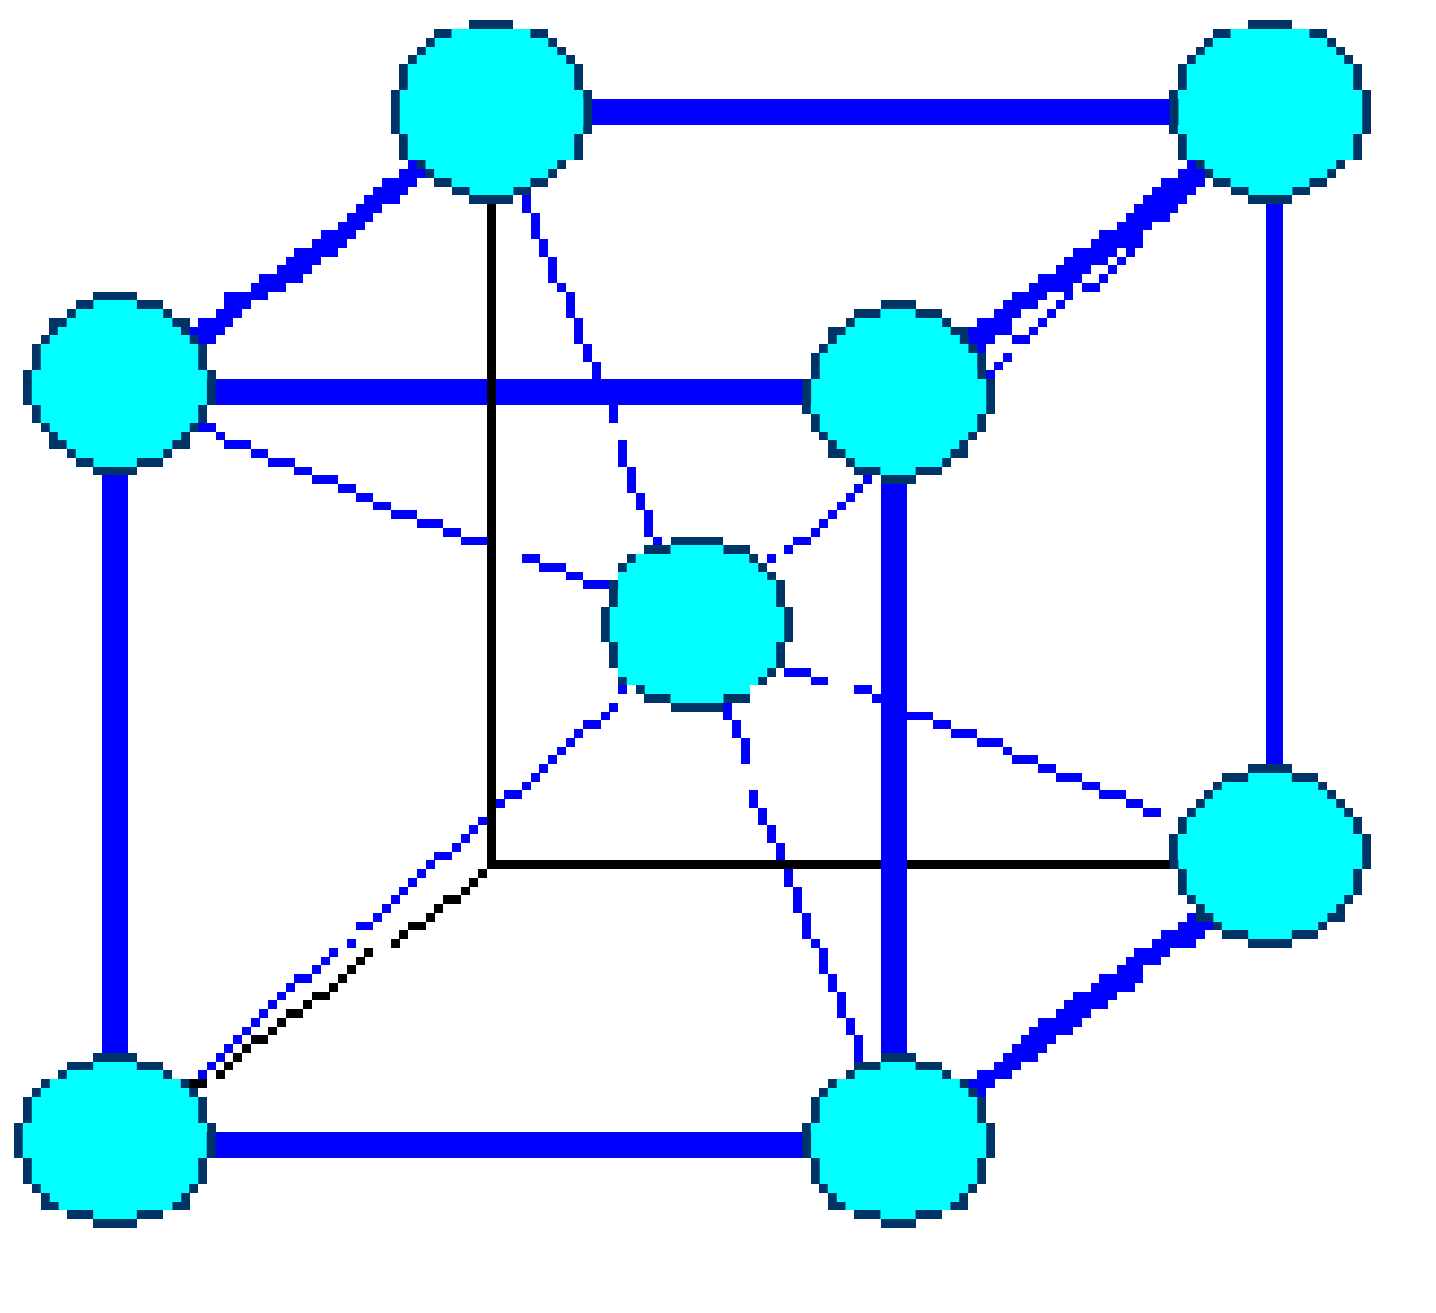
\includegraphics[width=0.5\linewidth]{images/1_krz.png}
		\caption{kubisch raumzentriert}
	\end{subfigure}
\end{figure}

\subsection{Packungsdichte}
Packungsdichte $P = \frac{V_{Atome}}{V_{Elementarzelle}}$, Raumerfüllung durch Atome einer Elementarzelle. Für dichteste Kugelpackungen ist $P=74\%$

\subsection{Gitterfehler}
\begin{itemize}
	\item Versetzung
	\item Unbesetzter Gitterplatz
	\item Fremdatom in Gitterlücke
	\item Fremdatom in Gitterplatz
\end{itemize}
\section{Atombau - Marco}

\subsection{Atome}
Atome bestehen aus Atomkern ($p^+$, $n$) und Atomhülle ($e^-$).

\begin{table}[htbp]
	\begin{tabular}{|l|c|c|}
		Elementarteilchen & Masse & El. Ladung \\ \hline
		Proton $p^+$ & 1.0073 u & 1+ \\
		Neutron $n$ & 1.0087 u & 0 \\
		Elektron $e^-$ & 0.0005 u & 1- \\ \hline
	\end{tabular}
\end{table}

Atomare Masseinheit $u$: $\frac{1}{12}$ der Masse eines C-12 Atoms. \\

Elementarladung $e$: $\pm 1.602 \cdot 10^{-19} C$ ($C$: Coulomb) \\

Schreibweise von Atomen: $ ^\text{Atommasse}_\text{Ordnungszahl} X ^\text{Ladung}$ \\

\subsection{Isotope}
Atome eines Elements, die sich in ihrer Neutronenzahl unterscheiden.

\subsection{Elektronen}
Elektronen befinden sich auf bestimmten, diskreten Energieniveaus (Schalen: K,L,M,N,...). 

\begin{figure}[htbp]
	\centering
	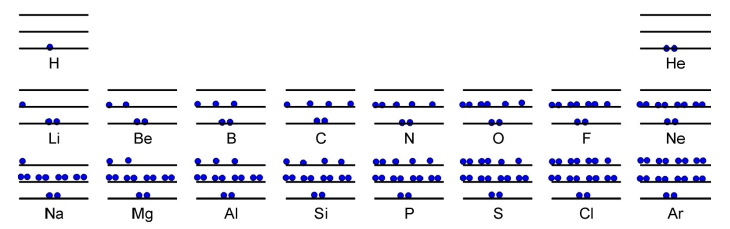
\includegraphics[width=0.9\linewidth]{images/2_Energie_der_Elektronen.png}
\end{figure}

Ionisierungsenergie $E_{Ion}$: Energie, welche benötigt wird um ein $e^-$ vollständig aus einem Atom zu entfernen.\\

Maximale Anzahl $e^-$ pro Energieniveau: $2 \cdot n^2$ (n: Nummer des Energieniveaus) \\

Valenzelektronen: Elektronen des höchsten Energieniveaus. Zahl der VE bestimmt chem. Eigenschaften eines Elements \\
Atomrumpf: Atom ohne Valenzelektronen \\
Rumpfladung: Ladung des Atomrumpfs \\

Energieniveaus werden aufgrund der Abstossung der $e^-$ in Unterniveaus (s,p,d,f,...) aufgeteilt. Unterniveaus verschiedener Hauptniveaus können sich überlappen (z.B. 4s liegt tiefer als 3d).

\subsection{Orbitalmodell}
Welle-Teilchen-Dualismus $\Rightarrow$ $e^-$ können als stehende Welle betrachtet werden. \\

Orbital: Raum, in dem sich ein $e^-$ mit grösster Wahrscheinlichkeit aufhält. \\

\subsubsection{Regeln für Elektronenkonfiguration}
\begin{enumerate}
	\item Besetzung der Orbitale mit $e^-$ nach aufsteigender Energie.
	\item Pauli-Prinzip: max. 2 $e^-$ pro Orbital.
	\item Hund'sche Regel: Orbitale mit gleicher Ordnung werden zuerst mit 1 $e^-$ besetzt.
\end{enumerate}

\begin{figure}[htbp]
	\centering
	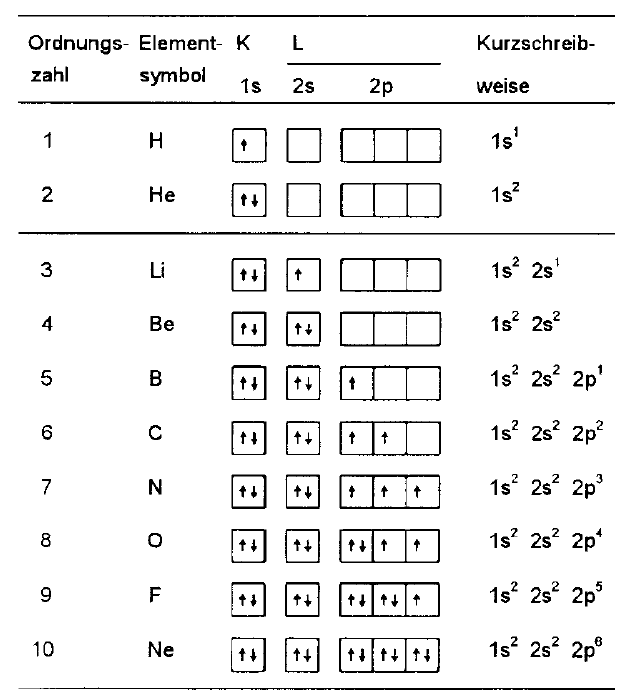
\includegraphics[width=0.75\linewidth]{images/2_Konfiguration_Orbitale.png}
\end{figure}

\subsection{Lewis-Schreibweise}
Meist spielen nur Valenzelektronen eine Rolle $\Rightarrow$ nur VE zeichnen.
\begin{figure}[htbp]
	\centering
	
\includegraphics[width=0.5\linewidth]{images/2_Lewis_Schreibweise.png}
\end{figure}

\subsection{Edelgasregel}
Alle Atome sind bestrebt eine Edelgaskonfiguration zu erreichen, d.h. 8 VE. Ausnahmen: H, He.

\begin{itemize}
	\item Metallatome: Abgabe von $e^-$ (kl. Rumpfladung) $\Rightarrow$ Kationen
	\item Nichtmetallatome: Aufnahme von $e^-$ $\Rightarrow$ Anionen, oder Teilen von $e^-$ mit anderen Atomen (Moleküle)
\end{itemize}
\section{Metalle}
Typische Eigenschaften: gute elektrische und Wärme-Leitfähigkeit, Duktilität, Glanz \\

\subsection{Elektronengas-Modell}
Metallkationen bilden ein Gitter, die VE sind delokalisiert (frei beweglich), weil Metalle kleine $E_{Ion}$ haben. \\

Metallische Bindung: ungerichtete elektrostatische Anziehung zwischen Metallkationen und $e^-$-Gas. \\

\subsection{Duktilität}
Reine Metalle sind relativ duktil, weil dichtest gepackte Schichten gut gegeneinander beweglich sind. Duktilität ist abhängig von der Zahl der Gleitebenen (d.h. Gittertyp, Korngrösse), der Stärke der metall. Bindung und der Gitterfehler. 

\subsection{Eisen}
\subsubsection{Aufbau}
\begin{figure}[htbp]
	\centering
	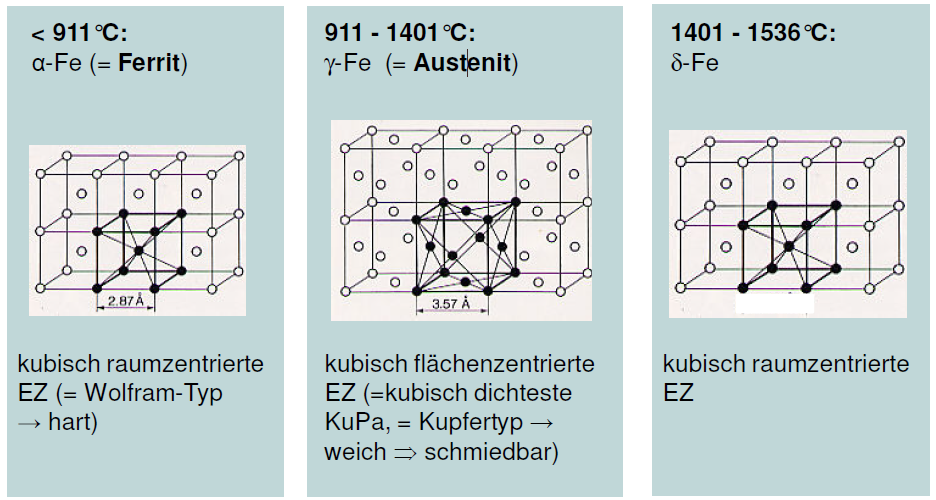
\includegraphics[width=0.9\linewidth]{images/3_Aufbau_Eisen.png}
\end{figure}

\subsection{Energiebänder-Modell}
Überlappung von $N$ Atomorbitalen (AO) führt zu N Molekülorbitalen (MO). Wenn N sehr gross $\Rightarrow$ Bänder aus MO $\Rightarrow$ elektrisch leitend.
\begin{itemize}
	\item Metalle: leeres Leitungsband überlappt mit (teilweise) gefülltem Valenzband
	\item Isolatoren: Grosse verbotene Zone zwischen Valenzband und Leitungsband
	\item Eigenhalbleiter: Kleine verbotene Zone
\end{itemize}

\subsubsection{Eisengewinnung}
Ausgangsstoffe: Fe-Erz, Koks, Zuschlagsstoffe (Kalk, Sand), Luft (O$_2$) \\

Prinzip: $Fe_xO_y + C \leftarrow Fe + CO_2$ \\

Gase: Durch Zuschlagsstoffe gebundene, unerwünschte Erze. \\
Gichtgas: Gase und Rest des Heisswinds. \\

Hochofenprozesse:
\begin{eqnarray*}
	C_{s} \quad &+ O_{2(g)} \quad &\rightarrow \quad CO_{2(g)} \\
	CO_{2(g)} &+ C_{(s)} & \rightarrow 2 CO_{g} \\
	Fe_2O_{3(s)} &+ 2 CO_{(g)} & \rightarrow 2 Fe_{(s)} + 2 CO_{2(g)} 
\end{eqnarray*}

\subsection{Legierungen}
Stoffe, die aus zwei oder mehr Elementen bestehen und metallische Eigenschaften aufweisen.

\begin{itemize}
	\item Substitutionslegierungen: gewisse Gitterplätze sind durch Fremdatome belegt. ($r_\text{Fremdatom} \approx r_\text{Basismetall}$). z.B. Ag-Au-Legierung, Cu$_3$Au
	\item Einlagerungslegierung: gewisse Gitterlücken sind durch Fremdatome belegt. ($r_\text{Fremdatom} \ll r_\text{Basismetall}$). z.B. Stahl, Zementit Fe$_3$C
\end{itemize}

\subsubsection{Eigenschaften}
\begin{itemize}
	\item Härte: Legierungen sind härter als reine Metalle. Ursache: Fremdatome behindern Gleitebenen.
	\item El. Leitfähigkeit: schlechtere leitend als Metalle. Ursache: Fremdatome behindern $e^-$-Fluss.
	\item Korrosionsbeständigkeit: meist korrosionsbeständiger als Metalle.
\end{itemize}

\subsection{Stahl}
\subsubsection{Frischen}
Verfahren zur Reduktion von C im Roheisen durch Einblasen von Sauerstoff. \\
Reaktionen:
\begin{eqnarray*}
	2 Fe + O_2 \quad &\rightarrow 2 FeO \\
	Mn + FeO &\rightarrow MnO + Fe \\
	Si + 2 FeO &\rightarrow SiO_2 + 2 Fe \\
	C + FeO &\rightarrow CO_{(g)}
\end{eqnarray*}

Je höher der C-Gehalt, desto fester und härter, aber spröder. Max. 2.06\% C ist in Eisen löslich. 

\subsubsection{Zusammensetzung}
Legierter Stahl enthält Fremdatome:

\begin{figure}[htbp]
	\centering
	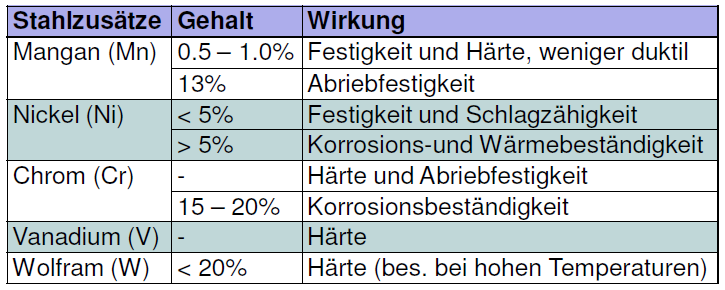
\includegraphics[width=0.9\linewidth]{images/3_Stahl_Zusaetze.png}
\end{figure}

\subsubsection{Eisen-Kohlenstoff-Zustandsdiagramm}
\begin{figure}[htbp]
	\centering
	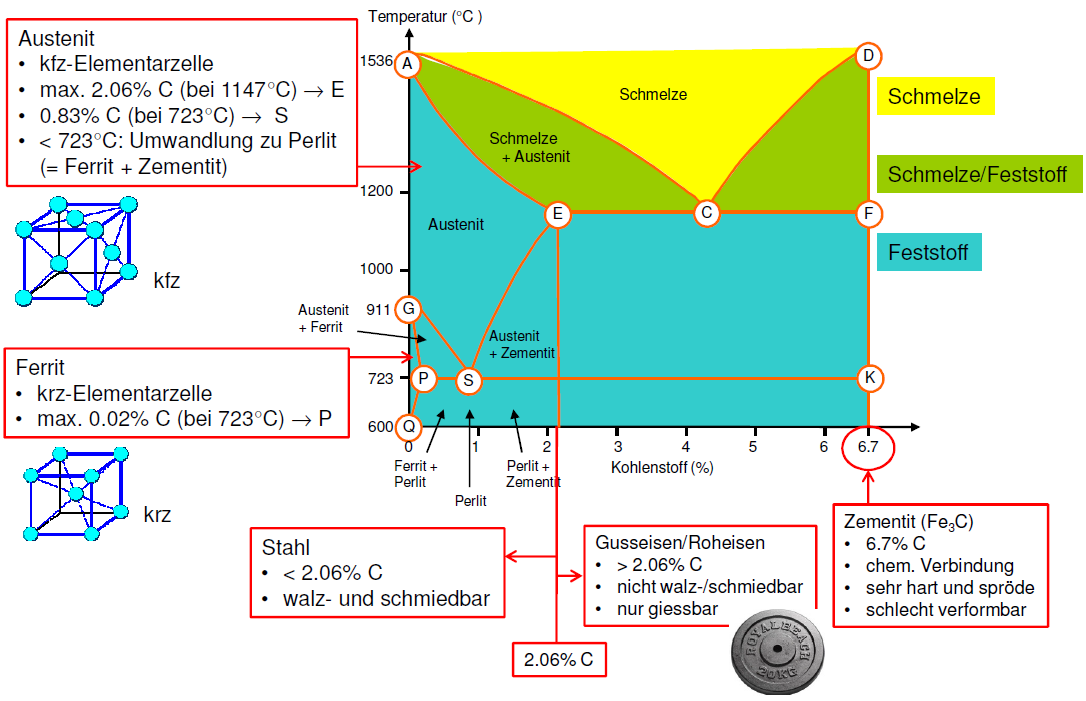
\includegraphics[width=0.95\linewidth]{images/3_Eisen_Kohlenstoff_Diagramm.png}
\end{figure}

\section{Halbmetalle und Halbleiter}
Halbmetalle: B, Si, Ge, As, Se, Sb, Te, Po, At \\

Halbmetalle zeigen keine einheitlichen Stoffeigenschaften und keinen einheitlichen Aufbau. \\

\subsection{Halbleiter}
Stoffe mit geringer el. Leitfähigkeit, welche bei steigender Temperatur zunimmt. Halbmetalle sind Halbleiter, aber nicht jeder Halbleiter ist ein Halbmetall. \\

Im Energiebänder-Modell: kleine Verbotene Zone zwischen Valenz- und Leitungsband, ca. 0-3 eV (Si: 1.12 eV bei 300K) \\

Bei steigender Temperatur: Zufuhr von Energie $\Rightarrow$ $e^-$ aus Valenzband kann ins leere Leitungsband springen und hinterlässt Lücke im Valenzband = \emph{Defektelektron}.

\begin{figure}[htbp]
	\centering
	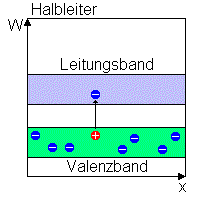
\includegraphics[width=0.4\linewidth]{images/4_Halbleiter_Energiebaender.png}
\end{figure}

\subsection{Dotierung}
Einbringen von Fremdatomen zur Veränderung der elektrischen Eigenschaften.

\subsubsection{n-Halbleiter}
El. Leitung v.a. durch $e^-$. \\

Bsp. Dotierung von Si mit As: 1 As-Atom pro $10^7$ Si-Atome. $\Rightarrow$ 1 schwach gebundenes Valenz-$e^-$ pro As-Atom $\Rightarrow$ Steigerung der Leitfähigkeit um Faktor $10^6$. \\

5. Valenz-$e^-$ entspricht einem vollen Energieband (Donatorband) knapp unterhalb des Leitungsbands. \\

\subsubsection{p-Halbleiter}
El. Leitung v.a. durch (positive) Defektelektronen. \\

Bsp. Dotierung von Si mit B: 1 B-Atom pro $10^6$ Si-Atome. $\Rightarrow$ 1 fehlendes $e^-$ pro B-Atom $\Rightarrow$ Defektelektron (\emph{Loch}) kann von Si-Valenz-$e^-$ besetzt werden $\Rightarrow$ positive Löcher. \\

Defektelektron entspricht leeren Energieband (Akzeptorband) knapp oberhalb des Valenzbandes.
\section{Molekulare Stoffe}
Moleküle sind abgeschlossene Atomverbände aus nichtmetallischen Atomen. 

\subsection{Bildung von Molekülen aus Atomen}
Atombindung (kovalente Bindung): Gemeinsames bindendes Elektronenpaar zwischen 2 Nichtmetallatomen. 

\subsubsection{Lewisformel}
\begin{multicols}{2}
$F_2$: \ \chemfig{\Lewis{0.246,F}+\Lewis{024.6, F}}  $\Rightarrow$  \chemfig{\Lewis{246,F}-\Lewis{026,F}} \\
$O_2$: \ \chemfig{\Lewis{0.246., O}+\Lewis{024.6., O}} $\Rightarrow$ \chemfig{\Lewis{35, O}=\Lewis{17, O}} \\
$N_2$: \ \chemfig{\Lewis{0.2.46., N}+\Lewis{02.4.6., N}} $\Rightarrow$ \chemfig{\Lewis{4, N}~\Lewis{0, N}} \\
$C_2Cl_2$: \ \chemfig{\Lewis{246, Cl}-[,0.7]C~[,0.7]C-[,0.7]\Lewis{026, Cl}}
\end{multicols}

\subsubsection{EPA-Modell}
Elektronenpaare stossen sich gegenseitig maximal ab. Damit kann die räumliche Struktur vorausgesagt werden. Bei vier Valenz-Kugelwolken beträgt der Winkel dazwischen $109.5^\degree$ (Tetraederwinkel).

\subsection{Elektronegativität (EN)}
Fähigkeit eines Atoms, Bindungselektronen anzuziehen. Die EN ist grösser, je grösser die Rumpfladung und je kleiner der Rumpfradius ist. $EN=\frac{Rumpfladung}{Rumpfgroesse}$

\subsection{Polare Bindung}
Polarität einer Bindung: $\Delta EN = | EN_{1} - EN_{2} |$. 
\begin{itemize}
	\item $\Delta EN = 0$: apolare Bindung
	\item $\Delta EN = 0 .. 1.5$: polare Bindung
	\item $\Delta EN > 1.5$: ionische Bindung
\end{itemize}

Moleküle sind Dipole (polare Moleküle), wenn die Schwerpunkte der Partialladungen nicht zusammenfallen.

\chemfig{\underset{3.0}{Cl}-\underset{3.0}{Cl}} $\Rightarrow \Delta EN=0$ apolare Bindung \\
\chemfig{\overset{\delta+}{\underset{2.1}{H}}-\overset{\delta-}{\underset{3.0}{Cl}}} $\Rightarrow \Delta EN=0.9$ polare Bindung \\
\chemfig{\underset{0.9}{Na^+}-\underset{3.0}{Cl^-}} $\Rightarrow \Delta EN=2.1$ ionische Bindung 

\subsection{Zwischenmolekulare Kräfte}
Anziehende Kräfte, die zwischen Molekülen herrschen und Stoffeigenschaften (mp,bp; Mischbarkeit; Viskosität; Oberflächenspannung; ...) beeinflussen. Normalerweise schwächer als kovalente Bindungen.

\begin{itemize}
	\item Dipol-Dipol Kräfte: gegenseitige Anziehung von Dipolmolekülen aufgrund unterschiedlicher Partialladungen. Je polarer, desto grösser.
	\item Van-der-Waals Kräfte: gegenseitige Anziehung von unpolaren Molekülen aufgrund kurzzeitig ungleichmässig verteilter Elektronen. Sehr schwach, mehr $e^-$ $\Rightarrow$ stärker, zwischen allen Molekülen
	\item Wasserstoffbrücken (H-Brücken): Anziehung zwischen stark positiv polarisierten H-Atomen und freien Elektronenpaaren von stark elektronegativen Atomen (F,O,N) $\Rightarrow$ existieren nur bei H-F, H-O oder H-N Bindungen. Stärkste zwischenmolekulare Kräfte.
\end{itemize}

\subsubsection{Siedepunkt abschätzen}
Prinzip: Beim Verdampfen müssen zwischenmolekulare Kräfte überwunden werden $\Rightarrow$ grosse zw.molek. Kräfte $\Leftrightarrow$ hoher Siedepunkt. 

\textbf{Beispiel:} Wasser bildet alle zwischenmolekularen Kräfte aus, das erklärt den höchsten Siedepunkt. $H_2Te$ bildet ausschliesslich VdW-Kräfte aus, weshalb der Siedepunkt eher tief ist.
\begin{figure}[htbp]
	\centering
	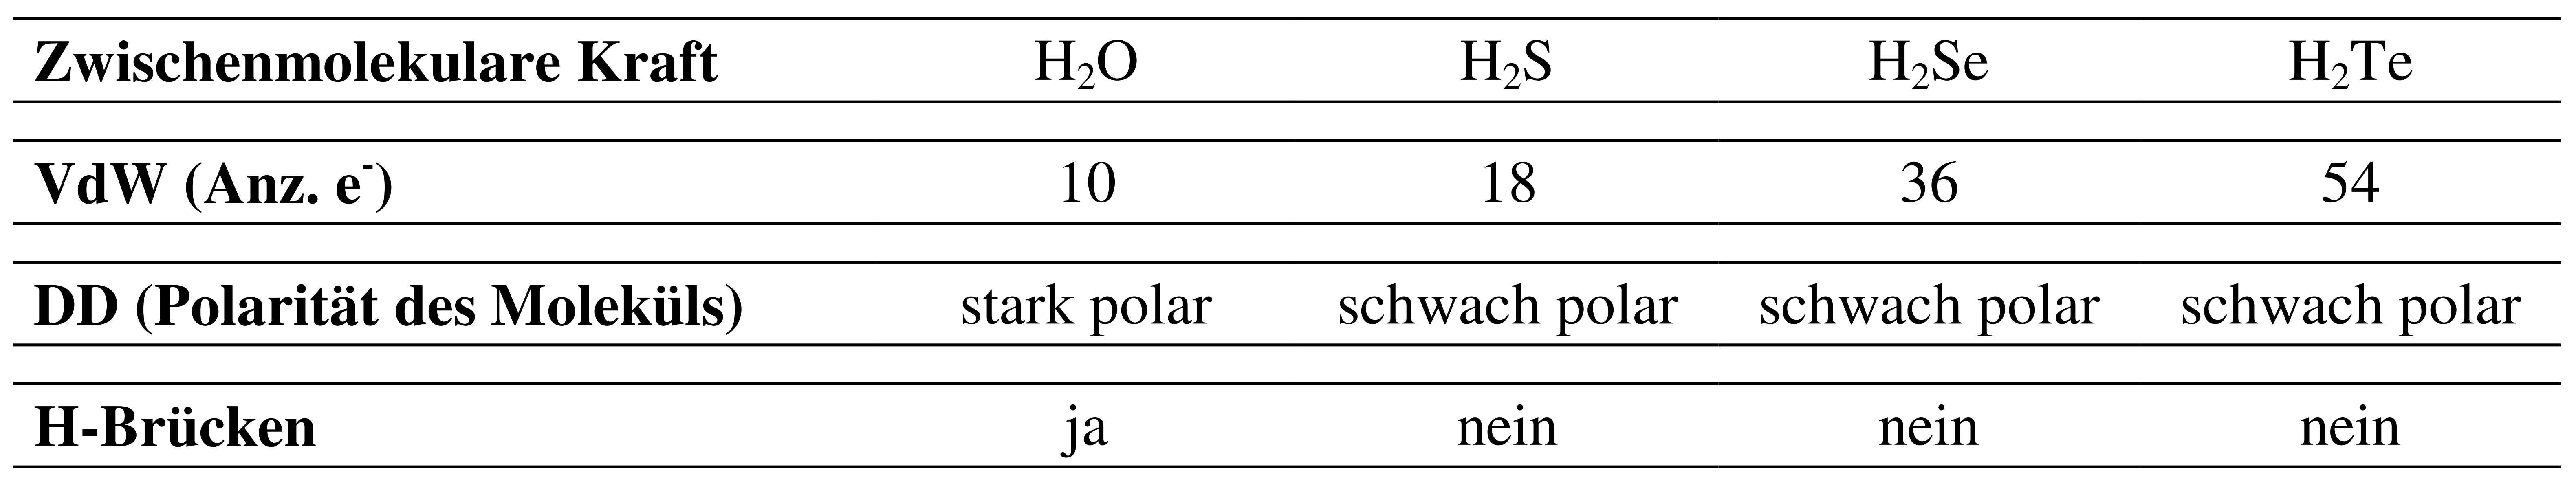
\includegraphics[width=1\linewidth]{images/5_Siedepunkt.png}
\end{figure}

\subsubsection{Löslichkeit abschätzen}
Prinzip: Ein molekularer Stoff ist löslich, wenn er mit dem Lösungsmittel dieselbe Art zwischenmolekularer Kräfte ausbilden kann. \\
Halbpolare Stoffe besitzen eine polare Gruppe (z.B. -OH) und einen nicht zu langen unpolaren Teil (z.B. KW-Kette). Je länger die KW-Kette desto hydrophober, schlechter löslich wird das Molekül.

\subsubsection{Zersetzung}
Bestimmte molekular aufgebaute Stoffe haben keinen Siedepunkt. Werden solche Stoffe erwärmt, zersetzen sie sich, d.h. Atombindungen im Molekül werden gebrochen und die Atome verknüpfen sich neu.

\subsection{Flüssigkristalle}
\subsubsection{Aggregatszustände}
\begin{itemize}
	\item fest: Moleküle mit 3-dimensionale Fernordnung, anisotrop (richtungsabhängig)
	\item flüssig: ungeordnete Moleküle, isotrop
	\item flüssigkristallin: Moleküle mit 1- oder 2-dimensionaler Fernordnung
\end{itemize}

\subsubsection{Phasen der Flüssigkristalle}
\begin{figure}[htbp]
	\centering
	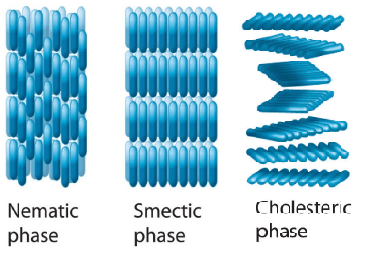
\includegraphics[width=0.5\linewidth]{images/11_Phasen.png}
\end{figure}
\begin{itemize}
	\item nemantische Phase
		\begin{itemize}
			\item 1-dimensionale Ordnung
			\item Moleküle entlang Längsachse ausgerichtet
			\item Molekülenden nicht geordnet
			\item Aneinander Vorbeigleiten möglich
		\end{itemize}
	\item smektische Phase
		\begin{itemize}
			\item 2-dimensionale Ordnung
			\item Moleküle entlang Längsachse ausgerichtet
			\item Molekülenden geordnet $\Rightarrow$ Entstehung von Schichten
			\item Aneinander Vorbeigleiten nicht möglich
			\item SmA: Längsachse in $90^\circ$-Winkel zur Schicht
			\item SmC: Längsachse geneigt zur Schicht
		\end{itemize}
	\item cholestrische Phase
		\begin{itemize}
			\item Schichten mit nematischer Ordnung
			\item jede Schicht um charakteristischen Winkel verdreht (Abstossungskräfte)
			\item Schraubenförmige (helikale) Struktur mit Periodizität im nm-Bereich.
		\end{itemize}
\end{itemize}

\subsection{Atomarer Aufbau}
Flüssigkristalle bestehen aus langen, stabartigen Molekülen mit starren Atomgruppen. 

\begin{figure}[htbp]
	\centering
	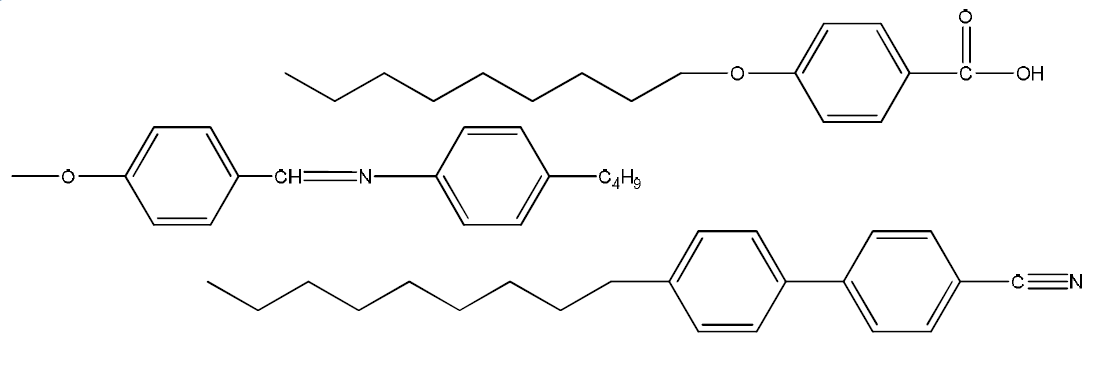
\includegraphics[width=0.8\linewidth]{images/11_Atome.png}
\end{figure}

Zwischenmolekulare Kräfte schränken die Beweglichkeit ein, die Stäbchen richten sich deshalb parallel aus. Da die Atomgruppen meist polar sind, entstehen Dipol-Dipol Kräfte und extern angelegte elektrische Felder können die Moleküle ausrichten (Prinzip des LCD Displays). 
\section{Salze}

\subsection{Aufbau}
Salzartige Stoffe bestehen aus Ionen (el. geladene Atome oder Moleküle). Zwischen den Ionen herrschen ungerichtete elektrostatische Kräfte.\\ Kationen $\Rightarrow$ oft Metallionen\\Anionen $\Rightarrow$ \emph{immer} Nichtmetallionen \\
Ionische Bindung: Elektrostatische Wechselwirkungen zwischen allen Kationen und Anionen. $F = \frac{1}{4 \pi \epsilon_0} \cdot \frac{Q_1 + Q_2}{d^2}$ \\
Kristalline Stoffe, oft in dichtester Kugelpackung angeordnet, (abhängig von Ionengrösse und Ionenverhältnis) z.B. NaCl-Typ:
\begin{figure}[h!]
	\centering
	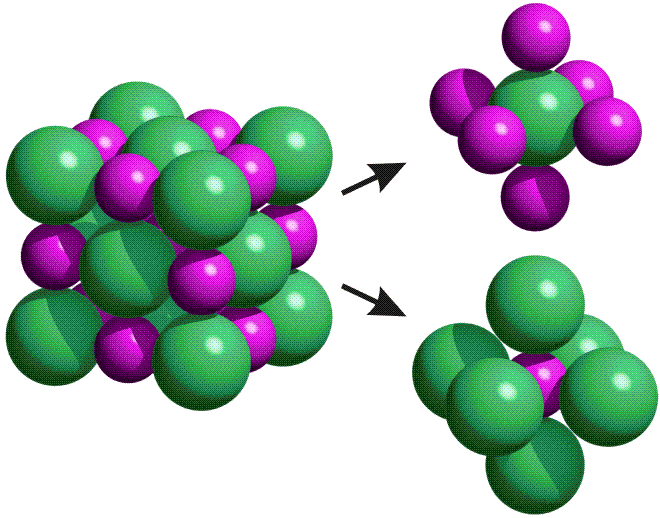
\includegraphics[width=0.4\linewidth]{images/5_Elementarzelle_NaCl.png}
\end{figure}

\subsection{Salzformeln}
Salzformeln sind Verhältnisformeln.
\begin{enumerate}[nolistsep]
	\item Die Ladungen der Ionen ergeben sich aus der Edelgasregel $\Rightarrow$ PSE: Hauptgruppe (HG) 1 bis 3 wollen $e^-$ abgeben, dh. Ionenladung = + HGNr.; HG 5 bis 7 wollen $e^-$ aufnehmen, dh. Ionenladung = - (8 - HGNr.)\\ 
	Bsp: Na $\Rightarrow$ Na$^+$, Al $\Rightarrow$ Al$^{3+}$ (möchte 3 e$^-$ abgeben), Cl $\Rightarrow$ Cl$^-$, O $\Rightarrow$ Na$^{2-}$ (möchte 2 e$^-$ aufnehmen)
	\item Salze sind insgesamt neutral. \\
	Bsp: Na $\Rightarrow$ Na$^+$: Cl$^-$ = 1:1  $\Rightarrow$  NaCl,\\
	Al$^{3+}$: O$^{2-}$ = 2:3 $\Rightarrow$ Al$_2$O$_3$
\end{enumerate}

\subsection{Nomenklatur}
Name Kation + (griech./lat.) Name Anion + \emph{-id} \\
Bei Übergangsmetallen: Kationenladung als römische Ziffer. 

\subsection{Gitterenergie}
$E_G$: Energie, um ein Salz in seine freien Ionen zu zerlegen (bzw. umgekehrt). Wird vor allem durch die Coulombkraft bestimmt. Wird umso grösser: je grösser die Ionenladungen und je kleiner die Ionenradien (Atomradien nehmen innerhalb einer Gruppe des PSE von oben nach unten zu und innerhalb einer Periode von links nach rechts ab) sind.

\subsection{Eigenschaften}
\subsubsection{Sprödigkeit}
Die Sprödigkeit sagt aus, wie stark sich ein Stoff verformen lässt bis er bricht. Bei Verformung eines Salzes müssen die Kationen- und Anionenebenen (durch eine externe Kraft) gegeneinander verschoben werden (so geraten Kationen neben Kationen und Anionen neben Anionen) $\Rightarrow$ Abstossung $\Rightarrow$ Bruch des Salzes

\subsubsection{Schmelz- und Siedepunkt}
Aufgrund der Coulumb-Kräfte, weisen Salze hohe Schmelz- (in der Regel über 400$^\circ$C) und Siedepkt. auf $\Rightarrow$ Sie sind somit schwerflüchtige (hoher Siedepkt.) Verbindungen. Schmelz(mp)- und Siedepkt.(bp) kann mit Hilfe der Gitterenergie abgeschätzt werden. D.h. je höher die Gitterenergie, desto höher der Schmelz- bzw. Siedepkt. 

\subsubsection{Elektrische Leitfähigkeit}
Feste Salze: keine elektrische Leitfähigkeit (el. Isolatoren); Salzschmelzen und Salzlösungen: gute Leitfähigkeit.\\
Die Leitfähigkeit einer Salzlösung ist abhängig von 3 Faktoren: Anionen- und Kationenkonzentrationen, Ladungszahlen der Anionen und Kationen, Beweglichkeiten der Anionen und Kationen

\subsubsection{Löslichkeit}
\begin{figure}[h!]
	\centering
	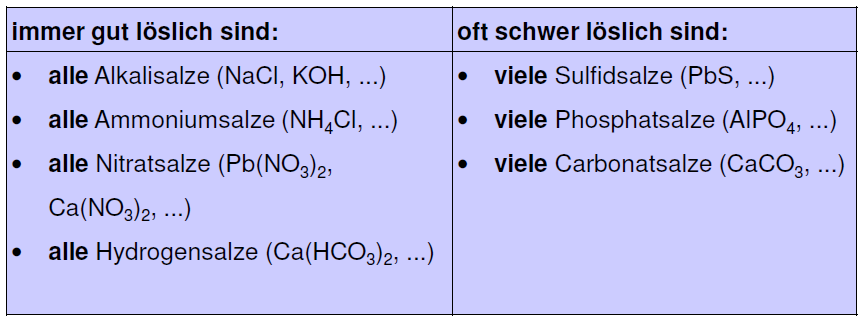
\includegraphics[width=0.9\linewidth]{images/5_Tabelle_Loeslichkeit.png}
\end{figure}
Sobald ein Salz mit einer polaren Flüssigkeit (z.B. Wasser) in Berührung kommt, ziehen die Ionen an der Oberfläche des Salzes die Dipolmoleküle an: Die negativen Pole ($\delta-$) der Dipolmoleküle werden von den Kationen, die positiven Pole ($\delta+$) von den Anionen angezogen. Temperaturschwingungen begünstigen das Eindringen von Dipolmolekülen zwischen Anionen und Kationen, was eine Schwächung der elektrostatischen Kräfte zur Folge hat. Die einzelnen Ionen können somit vollständig von Dipolmolekülen umhüllt werden und sich vom Salzkristall ablösen.

Schreibweise: $NaCl_{(s)} \, \rightarrow \, Na^+_{(aq)} + Cl^-_{(aq)}$
\section{Hochmolekulare Stoffe - Polymere - Lukas}
Hochmolekulare Stoffe bestehen aus sehr langen Molekülen, sog. \emph{Makromolekülen}, mit einer Molaren Masse von >10'000 g/mol. Makromoleküle lassen sich in kleine, sich wiederholende Abschnitte, \emph{Monomere}, unterteilen. \\

\subsection{Unterscheidung}
\begin{itemize}
	\item natürlich vorkommende hochmolekulare Stoffe, z.B. Baumwolle
	\item künstlich hergestellte hochmolekulare Stoffe (Kunststoffe)
		\begin{itemize}
			\item Thermoplaste (lineare oder verzweigte Makromoleküle)
			\item Duroplaste (engmaschig vernetzte Makromoleküle)
			\item Elastomere (weitmaschig vernetzte Makromoleküle)
		\end{itemize}
\end{itemize}

\begin{figure}[htbp]
	\centering
	\begin{subfigure}{0.25\linewidth}
		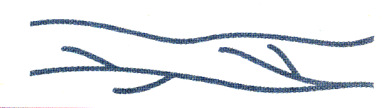
\includegraphics[width=0.9\linewidth]{images/7_Thermoplast}
		\caption{Thermoplast}
	\end{subfigure}
	\quad
	\begin{subfigure}{0.25\linewidth}
		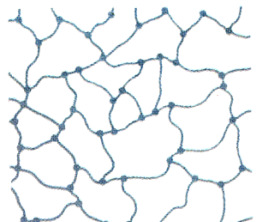
\includegraphics[width=0.9\linewidth]{images/7_Duroplast}
		\caption{Duroplast}
	\end{subfigure}
	\quad
	\begin{subfigure}{0.25\linewidth}
		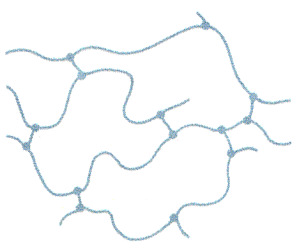
\includegraphics[width=0.9\linewidth]{images/7_Elastomer}
		\caption{Elastomer}
	\end{subfigure}
\end{figure}

\subsection{Eigenschaften}
\begin{itemize}
	\item geringe Dichte (0.8 bis 2 g/cm$^3$), weil Atome (v.a. C,H) geringe Masse haben.
	\item grosse chemische Beständigkeit, weil keine reaktionsfreudigen Gruppen.
	\item kein Siedepunkt, sondern Zersetzung, weil VdW-Kräfte oder Vernetzung
	\item sehr geringe elektrische und Wärme-Leitfähigkeit, weil keine geladenen, frei beweglichen Teilchen vorhanden
\end{itemize}

\subsection{Thermoplaste}
Bsp. Polyethen (PE), Polypropen (PP), Polyvinylchlorid (PVC), ... \\

Lineare oder verzweigte Makromoleküle. Länge: $0.001$ bis $1 \mu m$. Kettenlänge kann innerhalb des Polymers variieren. \\

Polymerisationsgrad: durchschnittliche Anzahl Monomere pro Makromolekül. \\

Thermoplaste sind teilkristallin, d.h. es können kristalline und amorphe Bereiche vorkommen.

\subsubsection{Taktizität}
Taktizität bezeichnet die räumliche Anordnung der Seitenketten / Fremdatome. Kann durch Herstellung beeinflusst werden.

\begin{figure}[htbp]
	\centering
	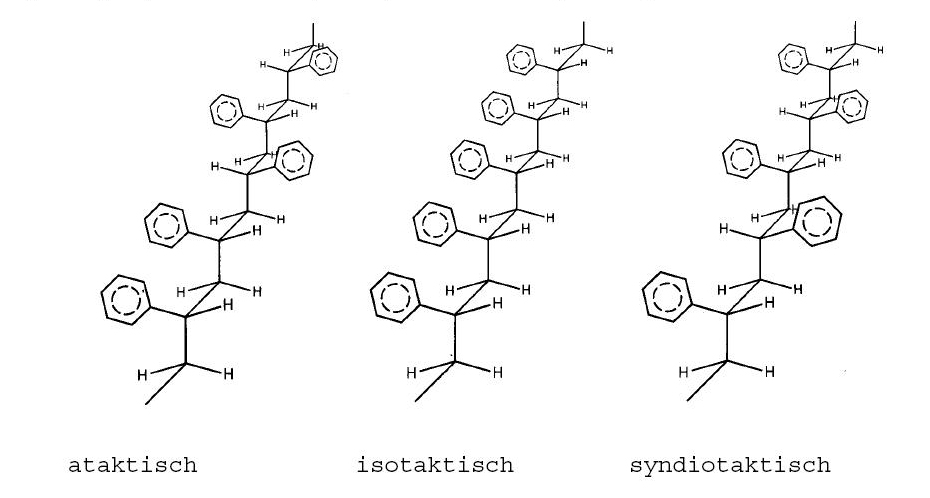
\includegraphics[width=0.7\linewidth]{images/7_Taktizitaet.png}
\end{figure}

\begin{itemize}
	\item ataktisch: amorphe Kunststoffe
	\item isotaktisch: hoher Kristallinitätsgrad möglich
\end{itemize}

\subsubsection{Eigenschaften}
\begin{itemize}
	\item schlecht löslich oder unlöslich (VdW-Kräfte)
	\item keinen Schmelzpunkt, sondern einen Schmelz\emph{bereich} (unterschiedlich starke VdW-Kräfte innerhalb)
	\item Durchlaufen beim Erwärmen versch. Aggregatzustände: fest $\rightarrow$ elastisch $\rightarrow$ plastisch $\rightarrow$ flüssig $\rightarrow$ Zersetzung
	\item Kristallinität beeinflusst Eigenschaften stark. Je kristalliner, desto höhere VdW-Kräfte
	\item Lange, unverzweigte Makromoleküle $\Rightarrow$ hohe Kristallinität, hohe Steifigkeit, hoher Schmelzbereich
\end{itemize}


\subsection{Duroplaste}
Bsp. Phenoplaste PF (Isoliermaterial, Steckdosen), Aminoplaste (Spannplattenleim), Ungesättigte Polyesterharze UP, Epoxidharze EP \\

Engmaschig vernetzte Makromoleküle $\Rightarrow$ hart, spröde, zerbrechlich, hitzebeständig (Netzstruktur bleibt beim Erwärmen erhalten) bis zur Zersetzung.

\subsection{Elastomere}
Bsp. Vernetze Polyurethane (PUR), Naturkautschuk (NR), Chloropren-Kautschuk (CR), Silikon-Kautschuk \\

Räumlich weitmaschig verknüpfte Makromoleküle $\Rightarrow$ elastisch, Zersetzung bei starkem Erwärmen.

\subsection{Herstellung von Polymeren}
Polymerisation: Verknüpfung der Monomere unter Spaltung einer Doppelbindung und Bildung einer neuen Einfachbindung $\Rightarrow$ kettenartige Makromoleküle $\Rightarrow$ Thermoplaste \\

Vulkanisation: Vernetzung von Makromolekülen mit Doppelbindungen. Ablauf: Zugabe von Schwefel $S_8$, Spaltung der $S_8$-Moleküle, Vernetzung der Makromoleküle, Produkt wird elastisch. 

\subsection{Verarbeitung von Polymeren}
Extrusion: Polymer-Granulat wird verflüssigt und mittels Druck in eine Form gepresst, z.B. Rohre, Schläuche. \\

Spritzgiessen: Wie Extrusion, jedoch wird das Polymer in eine fertige Form gespritzt, z.B. Tupperware, Kübel. \\

Blasformen: Rohling wird unter Druck und Temperatur innerhalb einer Form aufgeblasen, z.B. Getränkeflaschen. \\
\section{Atomgitter - Marco}

\subsection{Modifikationen des Kohlenstoffs}
Graphit: wabenförmige Schichten aus $C_6$-Ringen $\Rightarrow$ jedes Atom geht 3 Bindungen an, das 4. Valenz-$e^-$ ist delokalisiert. Zwischen den schichten herrschen VdW-Kräfte ($\Rightarrow$ weich). Eigenschaften: sehr weich, el. Leiter, metallischer Glanz.

\subsection{Diamantartige Stoffe}
Stoffe, die sehr hart sind, Bsp. Diamant $C_D$ (Mohs-Härte 10), Quarz $SiO_2$ (7), Korund $Al_2O_3$ (9) \\

Atomarer Aufbau sehr unterschiedlich. Diamant: Atomgitter mit kovalenten Bindungen, Quarz: Atomgitter mit kovalent-ionischen Bindungen, Korund: Ionengitter (d.h. ein Salz).

\subsection{Quarz ($SiO_2$)}
Si-Atome tetraedrisch, kovalent mit O-Atomen gebunden $\Rightarrow$ kovalent-ionische Bindungen. Aufbau ähnlich wie bei $C_D$. \\

Eigenschaften: el. Isolator, Härte 7, Schwingung bei Anlegen eines el.-mag. Feldes. \\

\subsection{Silikate}
Bsp. natürliche: Sand, Sandstein, Granit, Glimmer, Smaragd, Asbest; synthetische: Glas, Zement, Beton, Glaskeramik \\

\subsubsection{Atomarer Aufbau}
Aus $SiO_4^{x-}$ Tetraedern aufgebaut. \\

\begin{figure}[htbp]
	\centering
	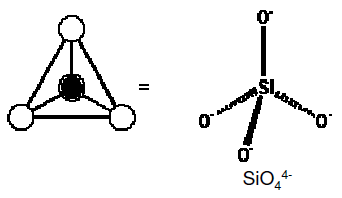
\includegraphics[width=0.4\linewidth]{images/8_SiO4.png}
\end{figure}

Unterschiedliche Verknüpfungen der Tetraeder ergeben verschiedene Silikate. Bsp. Gruppensilikat $Si_2O_7^{6-}$ (zwei Tetraeder), Ringsilikate (unterschiedlich grosse Ringe möglich), Kettensilikate, Bandsilikate  (siehe Bild unten), Schichtsilikate (Bandsilikate nebeneinander angeordnet)

\begin{figure}[htbp]
	\centering
	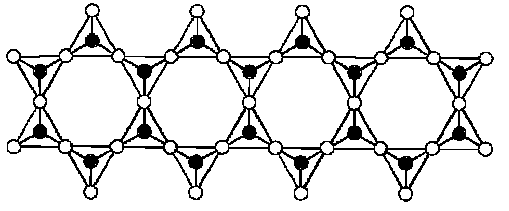
\includegraphics[width=0.7\linewidth]{images/8_Bandsilikat.png}
\end{figure}

3-dimensionales Atomgitter (Gerüstsilikat) $\Rightarrow$ $SiO_2$ Quarz

\subsubsection{Salzartige Silikate}
Nicht verknüpfte O-Atome sind an H oder $M^{a+}$ Kationen gebunden. Viele Minerale sind salzartige Stoffe mit Silikat-Anionen, z.B. Olivin, Aquamarin, Smaragd, Tonminerale (Ton, Talk), Glimmer. \\

Tonminerale sind sehr weich, leicht spaltbar und haben ein gutes Quellvermögen, weil diese aus durch VdW-Kräften zusammengehaltenen Silikatschichten bestehen. Entlang dieser Spalten sind die Tonminerale gut spaltbar oder es können Teilchen eingelagert werden. 

\subsection{Glas}
Gläser sind amorphe Stoffe. Bsp. Quarzglas: amorphes $SiO_2$ mit verzerrten Tetraedern.
\section{Redox-Reaktionen}
Redox-Reaktionen sind Elektronenübertragungs-Reaktionen. Dabei findet gleichzeitig eine Reduktion und eine Oxidation statt.

\subsection{Oxidation und Reduktion}
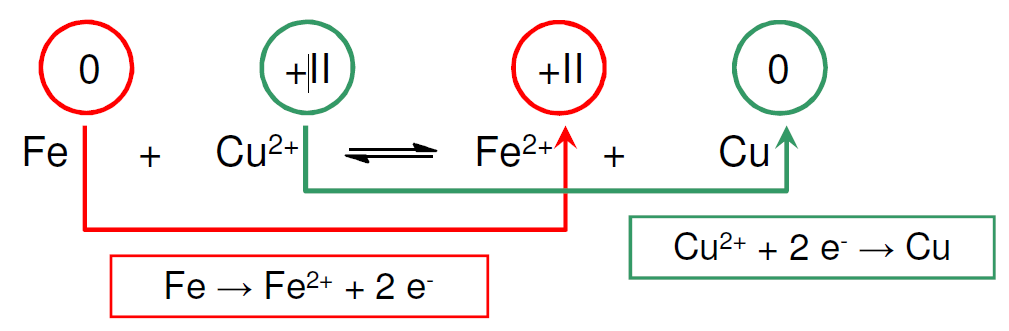
\includegraphics[width=0.6\linewidth]{images/9_Redox_Reaktion.png}\\
Oxidation (rot) = Elektronenabgabe, $X^m \Rightarrow X^{m+1} + e{^-}$\\
Bei der Oxidation wird die Oxidationszahl erhöht. Ein Reduktionsmittel (Elektronenspender) gibt Elektronen ab, dabei wird es oxidiert, es wird zum Oxidationsmittel (Elektronenakzeptor).\\
Reduktion (grün) = Elektronenaufnahme, $Y^n + e{^-} \Rightarrow Y^{n-1}$\\
Bei der Reduktion wird die Oxidationszahl reduziert. Ein Oxidationsmittel nimmt Elektronen auf, dabei wird es reduziert, es wird zum Reduktionsmittel.

\subsection{Oxidationszahlen (OZ)}
Um eine Redox-Reaktion erkennen zu können, muss man wissen, welcher Stoff $e^-$ aufnimmt (oxidieren) bzw. $e^-$ abgibt (reduzieren). Oxidationszahlen werden mit römischen Ziffern geschrieben. \\
Zur Bestimmung der OZ gelten folgende Regeln:
\vspace*{-0.1cm}
\begin{enumerate}[nolistsep]
	\item Die OZ der Atome in ihrer elementaren Form ist 0, Bsp. $O_2^0$, $Na^0$
	\item Bei einatomigen Ionen entspricht die OZ der Ionenladung (siehe Salze), Bsp. $Na^+$: OZ=+I
	\item Bei Molekülen werden die Bindungselektronen dem elektronegativeren Atom zugeordnet. \\
	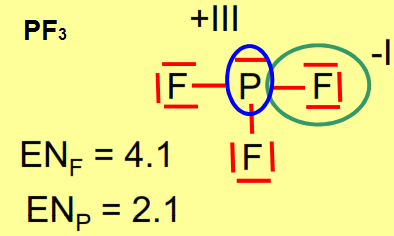
\includegraphics[width=4cm]{images/RedoxRegel3.png}\\
	Faustregeln: $F$ immer -I, $O$ fast immer -II, $H$ fast immer +I
	\item Die Summe aller OZ muss der Ladung des Teilchens entsprechen. Bsp: $H_3O^+$\\
	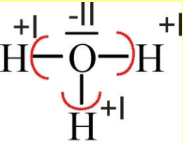
\includegraphics[width=2cm]{images/RedoxRegel4.png}
\end{enumerate}

\subsection{Vorhersage Brennbarkeit eines Stoffes}
Verbrennunsreaktionen sind Reaktionen mit Sauerstoff $O_2$. Dabei wirkt $O_2$ als Oxidationsmittel. Ein Stoff ist theoretisch brennbar, wenn er Elemente enthält, die noch nicht in der (für das jeweilige Element) höchsten Oxidationsstufe vorliegen. Dies kann man wie folgt prüfen:
\begin{enumerate}[nolistsep]
\item Oxidationszahlen mittels obigen Regeln bestimmen.
\item Prüfen ob bereits die höchste Oxidationsstufe eines Stoffes vorliegt (Abgleich mit PSE $\Rightarrow$ höchste positive Oxidationszahl). Falls ja, nicht brennbar, sonst brennbar!
\end{enumerate}

\subsection{Die Redox-Reihe}
Die Redox-Reihe gibt Auskunft über die Stärke eines Stoffs als Reduktions- bzw. Oxidationsmittels. Eine Redox-Reaktion kann ablaufen, wenn das Reduktionsmittel höher in der Tabelle liegt als das Oxidationsmittel. \\
Tabelle siehe Anhang. 

\subsection{Das Redox-Potential}
Das Redox-Potential beschreibt das Reduktions- bzw. Oxidationsvermögen einer Halbzelle (Redoxpaar) in Volt. In der Redox-Reihe ist für jedes Redoxpaar ein Standard-Redox-Potential (1 mol/l, 1013 mbar, 25$^\circ$C) aufgeführt. Redoxpaare mit einem hohen Elektronendruck sthen in der Redox-Reihe weit oben, sie haben ein negatives Redox-Potential. Umgekehrtes gilt für Paare mit einem tiefen Elektronendruck.

\subsubsection{Edle und unedle Metalle}
\emph{Edle} Metalle: $E^0 > 0V$, zeigen kaum Reaktion mit $O_2, H_2O$, Säuren. Kommen gediegen in der Natur vor. \\
\emph{Unedle} Metalle: $E^0 < 0V$, gehen mit vielen Stoffen Reaktionen ein. Kommen in der Natur nur in Form von Verbindungen vor. 

\subsubsection{Konzentrationsabhängigkeit des Redox-Potential}
Das Standard-Potential $E^0$ einer Halbzelle ist definiert für eine Ionen-Konzentration von 1 mol/l. Das effektive Redoxpotential wird gemäss der \emph{Nernst}-Gleichung beschrieben:
\begin{eqnarray*}
	E_{RM/OM} &= E^0_{RM/OM} + \frac{R \cdot T}{z \cdot F} \cdot \ln\frac{[OM]}{[RM]} \\ &=  E^0_{RM/OM} + \frac{0.059V}{z} \cdot \lg\frac{[OM]}{[RM]}
\end{eqnarray*}
mit der Gaskonstante $R=8.214\frac{J}{mol \cdot K}$, der Temperatur $T$ in $K$, der Faraday-Konstante $F=96485\frac{C}{mol}$ und der Zahl der übertragenen Elektronen pro Formeleinheit $z$ (aus Redox-Reihe). Zudem gilt, für feste Metalle (und andere unlösliche Stoffe) ist [RM] konstant und wird in der Nernstschen Gleichung = 1 gesetzt. \\
Generell: je kleiner die Konzentration, desto unedler das Redox-Potential.

\subsubsection{Die pH-Abhängigkeit des Redox-Potential}
Sind an einem Redoxpaar auch Protonen ($H^+$) beteiligt, so ist das Redox-Potential auch vom pH-Wert abhängig.\\
Redoxpaar $H_2 + 2 H_2O$ \& $2 H_3O^+ + 2 e^-$: \\ $E = -0.059V \cdot pH$ \\
Redoxpaar $4 OH^-$ \& $O_2 + 2 H_2O + 4 e^-$: \\ $E = 1.23 - 0.056V \cdot pH$ \\
Generell: je saurer (tiefer) der pH-Wert, desto edler das Redoxpotential. 



\section{Elektrochemie - Marco}

\subsection{Galvanische Zelle}
Grundprinzip: Oxidation und Reduktion sind räumlich getrennt. \\
Anode: Ort der Oxidation \\
Kathode: Ort der Reduktion \\

Daniell-Element:
\begin{figure}[htbp!]
	\centering
	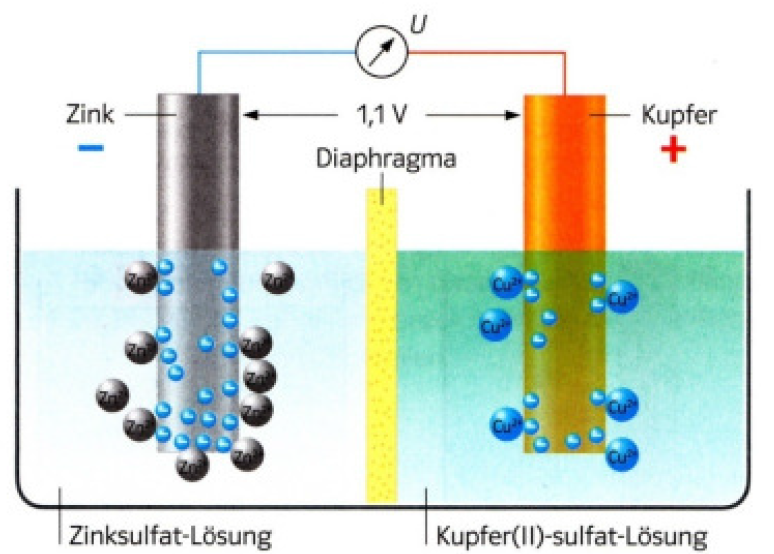
\includegraphics[width=0.7\linewidth]{images/10_Daniell_Element.png}
\end{figure}

Spannung $\Delta E = E_\text{Kathode}-E_\text{Anode}$ \\

Reaktionen:\\
Zink-Halbzelle (Anode): $Zn \leftrightarrow Zn^{2+} + 2 e^-$ \\
Kupfer-Halbzelle (Kathode): $Cu^{2+} + 2 e^- \leftrightarrow Cu$ \\

\subsubsection{Standard-Wasserstoffelektrode}
Referenzmessung des Redoxpotentials

\begin{figure}[htbp!]
	\centering
	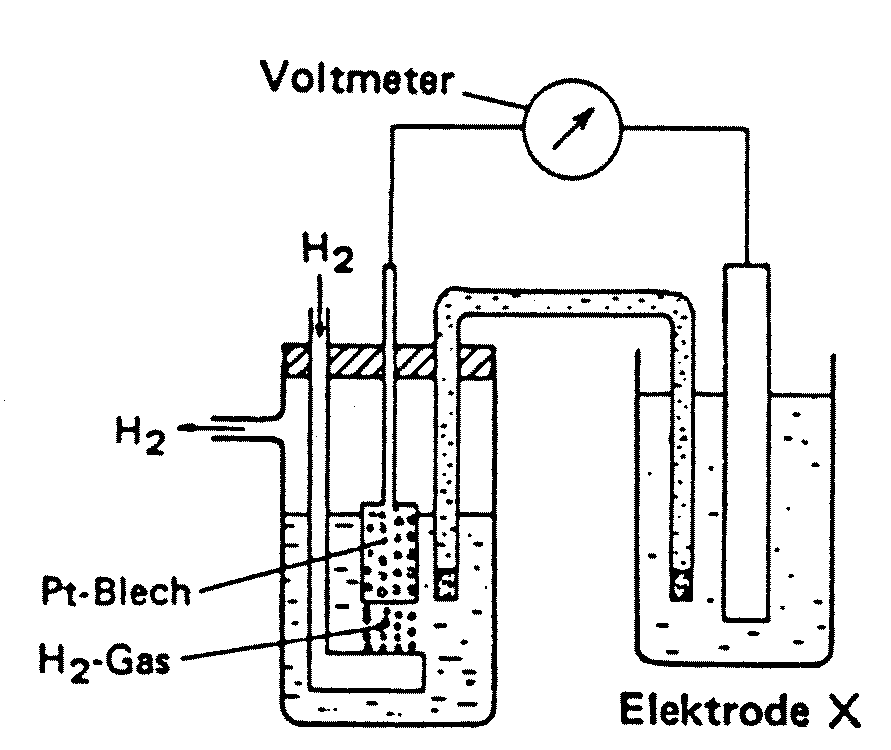
\includegraphics[width=0.6\linewidth]{images/10_Wasserstoffelektrode.png}
\end{figure}

Standardbedingungen:\\
p($H_2$) = 1013mbar, T=25$^\circ C$, Konzentration $[H_3O^+]$ = 1mol/l, $E^0(H_2/H_3O^+) = 0.0V$

Reaktionen: \\
Wasserstoff-Halbzelle: $H_2 + 2H_2O \leftrightarrow 2 H_3O^+ + 2 e^-$ \\
Halbzelle: $Me^{z+} + z e^- \leftrightarrow Me_{(s)}$ \\


\subsection{Edle und unedle Metalle}
\emph{Edle} Metalle: $E^0 > 0V$, zeigen kaum Reaktion mit $O_2, H_2O$, Säuren. Kommen gediegen in der Natur vor. \\

\emph{Unedle} Metalle: $E^0 < 0V$, gehen mit vielen Stoffen Reaktionen ein. Kommen in der Natur nur in Form von Verbindungen vor. \\

\subsection{Konzentrationsabhängigkeit des Redoxpotentials}
Das Redoxpotential ist u.a. von Temperatur, Druck, pH-Wert und Ionenkonzentration der Lösung vor. Das effektive Redoxpotential wird gemäss der \emph{Nernst}-Gleichung beschrieben:
\begin{eqnarray*}
	E_{RM/OM} &= E^0_{RM/OM} + \frac{R \cdot T}{z \cdot F} \cdot \ln\frac{[OM]}{[RM]} \\ &=  E^0_{RM/OM} + \frac{0.059V}{z} \cdot \lg\frac{[OM]}{[RM]}
\end{eqnarray*}
mit der Gaskonstante $R=8.214\frac{J}{mol \cdot K}$, der Temperatur $T$ in $K$, der Faraday-Konstante $F=96485\frac{C}{mol}$ und der Zahl der übertragenen Elektronen pro Formeleinheit $z$. \\

Generell: je kleiner die Konzentration, desto unedler das Redoxpotential. \\

Daraus ergibt sich für Halbzellen, in welche $H^+$ oder $OH^-$ vorkommen eine Abhängigkeit vom pH-Wert: \\
Redoxpaar $H_2 + 2 H_2O | 2 H_3O^+ + 2 e^-$: \\ $E = -0.059V \cdot pH$ \\
Redoxpaar $4 OH^- | O_2 + 2 H_2O + 4 e^-$: \\ $E = 1.23 - 0.056V \cdot pH$ \\

Generell: je saurer (tiefer) der pH-Wert, desto edler das Redoxpotential. \\

\subsection{Primärelemente}
Primärelemente sind galvanische Zellen, welche nach der Entladung nicht erneut aufgeladen werden können.

\subsubsection{Zink-Braunstein-Zelle}
\begin{table}[htbp]
	\begin{tabular}{lll}
	Anode (-) & $Zn$ \\ &\quad  $\rightarrow$ $Zn^{2+} + 2 e^-$ \\
	Kathode (+) & $2 MnO_2 + 2 H_3O^+ + 2e^-$ \\ &\quad $\rightarrow$ $2 MnO(OH) + 2 H_2O$  \\ \hline
	Gesamt & $Zn + 2 MnO_2 + 2 H_3O^+$ \\ &\quad $\rightarrow$ $2 MnO(OH) + Zn^{2+} + 2 H_2O$
	\end{tabular} 
\end{table}


Spannung: \\
Anode: $E^0 = -0.76V$ \\
Kathode: $E^0 = +0.74V$ \\
$\Rightarrow \Delta E = 1.5V$\\

Elektrolyt: eingedickte $NH_4Cl$-Lösung (sauer). Dieses wirkt gleichzeitig als Diaphragma.\\

Nachteile: nicht auslaufsicher, nicht hochstrombelastbar, hohe Selbstentladung \\

\subsubsection{Alkali-Mangan-Batterie}
Gleiche Reaktion wie bei Zink-Braunstein-Zelle. Elektrolyt: Kalilauge ($KOH
$, alkalisch). Vorteile: auslaufsicherer, günstigeres Entladeverhalten, pro $Ah$ ca. halb so teuer.

\subsection{Sekundärelemente}
Sekundärelemente können erneut aufgeladen werden (Akkumulator).

\subsubsection{Blei-Akkumulator}
Aufbau: 2 Sätze von Blei-Platten ineinander geschoben. Trennwand (Scheider) verhindert Berührung. Schwefelsäure-Lösung als Elektrolyt. Serieschaltung von 6 Zellen. \\

Vorbehandlung: Pb bildet in Schwefelsäure-Lösung eine festhaftende Sulfatschicht: \\

\begin{table}[htbp]
	\begin{tabular}{llll}
		Oxidation: & $Pb$ & $\rightarrow$ & $Pb^{2+} + 2 e^-$ \\
		Reduktion: & $2 H_3O^+ + 2 e^-$ & $\rightarrow$ & $H_2 + 2 H_2O$ \\ \hline
		Redox: & $Pb + 2 H_3O^+$ & $\rightarrow$ & $Pb^{2+} + H_2 + 2 H_2O$ \\
		mit $SO_4$: & $+ SO_4^{2-}$ & & $+ SO_4^{2-}$ \\ \hline
		Gesamt: & \multicolumn{3}{l}{$Pb + 2 H_3O^+ + SO_4^{2-}$} \\
		& \multicolumn{3}{l}{\qquad $\rightarrow$ $PbSO_4 + H_2 + 2 H_2O$} \\
	\end{tabular}
\end{table}


Lade-/Entladereaktion: \\
\begin{equation*}
	2 PbSO_4 + 2 H_2O \leftrightarrow Pb^0 + PbO_2 + 2 H_2SO_4
\end{equation*}

Zersetzungsspannung: $EMK = 2.05V$ \\

Aufladen des Akkus: Elektrolyse mit $PObSO_4$-Elektroden. \\
Entladen des Akkus: Rückreaktion des Ladevorgangs. \\

Elektrolytische Wasserzersetzung: \\
Anode: $6 H_2O \rightarrow O_2 + 4 H_3O^+ +  3e^-$ \\
Kathode: $4 H_3O^+ + 4 e^- \rightarrow 2 H_2 + 4 H_2O$ \\
Gesamtreaktion: $2 H_2O \rightarrow 2 H_2 + O_2$ \\

mit $U_z(H_2O) = \Delta E = 1.23V$. \\

Es findet jedoch keine $H_2O$-Zersetzung statt, weil eine hohe Überspannung ($U_{\ddot{u}} = U_Z-EMK=0.82V)$ nötig wäre. Es kann aber bei vollständiger Ladung zu Ausgasung kommen wobei Knallgas entsteht ($H_2,O_2$).

\subsubsection{Lithium-Ionen-Akkumulator}
Anode: Li-Atome, in Graphit eingelagert \\
Kathode: pulverförmiges Li-Metalloxid (ein Salz) \\
Elektrolyt: organisches Lösungsmittel mit gelöstem Li-Salz. \\

Entladereaktionen:
\begin{table}[htbp]
	\begin{tabular}{ll}
		Anode (-): & $Li$ \\ &\qquad $\rightarrow$  $Li^+ + e^-$ \\
		Kathode (+): & $Li_{x-1}Co^{+IV}O_2 + Li^+ + e^-$ \\ &\qquad $\rightarrow$ $Li_xCo^{+III}O_2$ \\ \hline
		Gesamt: & $Li + CoO_2$ \\ &\qquad $\rightarrow$  $LiCoO_2$
	\end{tabular}
\end{table}

$Li^+$ wandert von Anode zur Kathode, wo es in das Metalloxid eingelagert wird. $e^-$ wandert via Elektronenleiter von Anode zur Kathode, wo es $Co$ reduziert. \\

Vorteile: hohe Energiedichte, hohe Zellspannung (3.6V), geringe Selbstentladung. \\

\subsection{Wasserstoff-Brennstoffzelle}
Prinzip einer Brennstoffzelle: Galvanische Zelle, bei der das OM und das RM kontinuierlich von aussen zugeführt werden. \\

\begin{figure}[htbp]
	\centering
	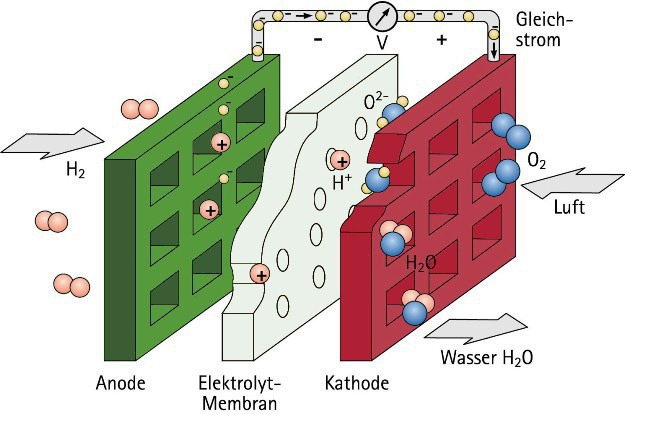
\includegraphics[width=0.6\linewidth]{images/10_Wasserstoffzelle.png}
\end{figure}

Reaktionen der $H_2$-Brennstoffzelle:
\begin{table}[htbp]
	\begin{tabular}{llll}
		Anode (-): & $H_2$ & $\rightarrow$ & $2 H^+ + 2 e^-$ \\
		Kathode (+): & $\frac{1}{2} O_2 + 2 e^-$ & $\rightarrow$ & $O^{2-}$ \\ \hline
		Gesamt: & $H_2 + \frac{1}{2} O_2$ & $\rightarrow$ & $H_2O$
	\end{tabular}
\end{table}

Spannung: \\
$E_{H2/H+} = -0.06V \cdot pH$ \\
$E_{H2O/O2} = 1.23V - 0.06V \cdot pH$ \\
$\Rightarrow \Delta E = 1.23 V$ \\

Aufbau einer polymer elektrolyte fuel cell (PEFC):
\begin{itemize}
	\item Polymermembran als Elektrolyt
	\item Elektroden aus Graphit
	\item Katalysatoren (Pt für Kathode, Pt/Ru für Anode)
	\item Gasdiffusionslage (GDL): poröses Graphitgeflecht für Verteilung der Gase, $e^-$-Leitung und Abtransport des $H_2O$
	\item Bipolarplatten aus Metall oder Graphit für Gaszuführung
\end{itemize}

\end{document}
